\documentclass{ieeeaccess}

\usepackage{cite}
\usepackage{amsmath,amssymb,amsfonts}
\usepackage{graphicx}
\graphicspath{{figures/}}
\usepackage{booktabs}
\usepackage{tabularx}
\usepackage{array}
\usepackage{url}
\usepackage[hidelinks]{hyperref}

% Keep short columns from stretching paragraph gaps across the page.
\raggedbottom

\newcommand{\Htwo}{H$_2$}
\newcommand{\NHthree}{NH$_3$}
\newcommand{\LHtwo}{LH$_2$}
\newcommand{\LOHC}{LOHC}
\newcommand{\DCR}{DCR}

\begin{document}

\history{Manuscript prepared September 7, 2026.}
\doi{}

\title{A Decision Support Tool for Prioritizing Hydrogen Import Interface Verification with Public European Infrastructure Data}

\author{\uppercase{Ruojun Duan}\authorrefmark{1}, AND \uppercase{Junjie Zhang}\authorrefmark{2,3}}

\address[1]{School of Political Science and International Relations, Tongji University, Shanghai 200092, China (e-mail: duanruojun@tongji.edu.cn)}
\address[2]{Shanghai Academy of Global Governance \& Area Studies, Shanghai International Studies University, Shanghai 201620, China (e-mail: junjiezhang2024@shisu.edu.cn)}
\address[3]{School of Economics and Finance, Shanghai International Studies University, Shanghai 201620, China}

\tfootnote{ORCID identifiers: Ruojun Duan: \href{https://orcid.org/0009-0008-6171-9373}{0009-0008-6171-9373}; Junjie Zhang: \href{https://orcid.org/0009-0004-8821-4018}{0009-0004-8821-4018}.}

\markboth{Duan and Zhang: Hydrogen Interface Verification Tool}{Duan and Zhang: Public Data Corridor Screen}
\corresp{Corresponding author: Junjie Zhang (e-mail: junjiezhang2024@shisu.edu.cn).}

\begin{abstract}
At the pre feasibility stage, port and hydrogen network planners must decide which announced import interfaces should be verified first when endpoint, capacity, status, and carrier compatibility records are incomplete. This paper presents a decision support protocol for producing a ranked verification shortlist, scenario specific flow allocations, and evidence gap diagnostics from public infrastructure data. The protocol combines a directed project graph, carrier compatibility rules, shared capacity pools by country and carrier, facility level demand accounting, and a two stage lexicographic scenario based robust mixed integer linear program (MILP). The frozen data product contains 69 nodes, 356 directed backbone edges, 22 explicit terminal interfaces, 20 carrier project records, and 55 industrial facilities. Twelve planning scenarios combine 2030/2040 horizons, PCI/PMI and Advanced infrastructure levels, and low, medium, and high EHO demand envelopes. An exact census of 126 four interface portfolios selects Belgium, Germany, northern France, and the Netherlands, with a 55.72\% worst planning scenario demand curtailment rate versus a 77.89\% median and a 100\% 90th percentile across the equal budget census. Removing capacity evidence increases N--1 failure stress by 22.11 percentage points, identifying capacity documentation as the first evidence collection priority in this product. The selected portfolio has a 77.89\% worst N--1 curtailment and a 92.38\% worst N--2 curtailment; these values provide verification stress diagnostics for the declared scenario set. The resulting priority set provides a bounded, auditable starting point for detailed engineering verification and subsequent planning studies.
\end{abstract}

\begin{keywords}
hydrogen infrastructure, import terminals, scenario based robust screening, mixed integer linear programming, project graphs, public data, engineering decision support
\end{keywords}

\titlepgskip=-21pt
\maketitle

\section{Introduction}
\label{sec:introduction}

\PARstart{H}{ydrogen} import planning is a coupled infrastructure problem. A carrier project must have an evidenced interface with a terminal, the terminal must connect to an identified hydrogen network node, the network must have a directed path to a demand location, and all of these elements must be available in the selected planning horizon. A large nominal import number is not a feasible service quantity when one of these links is missing. This distinction matters for European planning because public sources describe a mixture of announced projects, scenario capacities, candidate infrastructure, and demand envelopes, but rarely provide observed terminal throughput, queueing, firm contracts, local pipe constraints, or project finance \cite{EC_REPowerEU,REDIII,HydrogenRegulation,HydrogenDirective,TENE,FuelEUMaritime}.

This paper asks an engineering question that can be answered with the available evidence: \emph{Which missing interface evidence creates the largest planning regret, and how can a port or hydrogen network planner identify that evidence with a reproducible public data screen?} The output is a priority verification set and a scenario specific flow allocation. The scope statement below defines the evidence, decision, and application boundary before the results are discussed. The output supports verification planning and subsequent detailed design, operations, and finance studies.

At the pre feasibility stage, the planner's practical question is narrower and more actionable: which terminal and backbone interfaces should receive the next limited verification effort, and how much could the planning screen change if a named evidence layer is wrong or unavailable? The answer must preserve endpoint provenance, respect documented capacity pools, and remain inspectable by a port or network engineering team.

The paper makes four contributions for this planning task.

\begin{enumerate}
    \item It delivers an auditable public data inventory that links explicit terminal interfaces, TYNDP hydrogen network edges, carrier project records, and EHO industrial facilities. Records without endpoints, capacities, status, or compatibility evidence are excluded and entered in an exclusion ledger.
    \item It provides a two stage lexicographic scenario based robust mixed integer linear program (MILP) for priority ranking. Binary variables identify interfaces for verification; continuous recourse variables allocate hydrogen equivalent flows for each declared scenario. Shared carrier pools prevent one anonymous project record from being counted at multiple terminals.
    \item It embeds a validation suite comprising an exact equal budget portfolio census, structural ablations, N--1 and N--2 failure analyses, capacity sensitivity, direct ammonia boundary checks, and an external TYNDP Hydrogen corridor face check.
    \item It demonstrates a positive engineering result. The tool identifies a four interface verification set, detects a 22.11 percentage point planning stress increase when capacity evidence is removed, and passes all predefined diagnostic gates. The output is a transparent priority list for what if planning.
\end{enumerate}

The central design choice is to treat public data incompleteness as an auditable model input rather than as a reason to insert a national centroid or an unverified inland capacity proxy. The intended use is the pre feasibility stage: a planner loads a versioned inventory, specifies the declared demand and infrastructure scenarios, obtains a priority verification list and stress diagnostics, and reruns the screen as endpoint or capacity evidence improves. The tool is therefore relevant to port planners, hydrogen network developers, and system planners who need a transparent first screen before commissioning detailed engineering studies.

\section{Related Work and Contribution}
\label{sec:related}

Carrier studies show that ammonia, liquid hydrogen, and \LOHC{} differ in conversion losses, transport distance, storage needs, terminal equipment, scale, technology readiness, and end use compatibility \cite{Raab2021,Johnston2022,Lee2022,Sterner2024,RestelliNH3,RestelliLH2,Spatolisano2024,Peecock2024,Wolf2024}. European supply chain studies add spatial infrastructure, inland transport, and industrial demand to this comparison \cite{Ganter2024,Kountouris2024,Eissler2025,Rey2025,GanterESNT2025}. Network formulations further show that the topology used in a hydrogen model changes the set of feasible allocations \cite{He2021,Jiang2022}.

Recent applications of optimization and spatial screening methods have established the relevance of ports, hydrogen hub selection, and mixed integer capacity allocation in energy infrastructure planning. Sadiq \emph{et al.} review greener seaport infrastructure and energy efficiency challenges; Paula \emph{et al.} combine GIS and Fuzzy AHP for clean hydrogen hub identification; and Luo \emph{et al.} formulate capacity allocation for a hydrogen integrated energy system with trading and storage \cite{Sadiq2021,Paula2025,LuoHIES2023}. These studies inform the present focus on spatial infrastructure screening. The present study adds an evidence and validation layer for interface verification under incomplete public records: the workflow preserves endpoint and capacity provenance, applies carrier compatibility before flow allocation, and evaluates whether an equal budget verification set remains informative when evidence is withheld.

Robust optimization provides the conceptual basis for a common first stage decision under adverse conditions \cite{BertsimasSim,BenTalRobust}. This study implements that idea as scenario based robust screening over a fixed finite scenario matrix. The framework translates the principle into an auditable engineering workflow: it makes data provenance and exclusions explicit, prevents anonymous capacity duplication, and tests whether the resulting priority set separates equal budget portfolios while remaining sensitive to missing evidence. Its contribution is a data and decision support capability within the declared product, with the application scope defined in the following statement.

\noindent\textbf{Scope and intended use.} This artifact is a pre feasibility screening protocol for limited verification resources. It returns a ranked shortlist of terminal and backbone interfaces, an evidence gap ranking, and scenario specific flow allocations and capacity ratios for engineering review. Binary variables encode verification priority for documented interfaces. Records lacking usable endpoints, capacity, status, or compatibility evidence are excluded or pooled conservatively; no national centroid interpolation or silent imputation is used. The scenario based robust result is a common screen over the declared scenario set, and failure outputs are stress diagnostics. Named terminal crosswalks, firm capacity records, local delivery routes, temporal constraints, and commercial data belong to subsequent engineering studies.

\section{Public Data Product and Evidence Definition}
\label{sec:data}

\subsection{Frozen sources}

The core infrastructure vintage is ENTSOG TYNDP 2024. Its public downloads, hydrogen infrastructure levels, IGI material, project records, and capacity tables define the network and project evidence used in the main experiment \cite{ENTSOGDownloads,ENTSOGInfraLevels,ENTSOGIGI,ENTSOGAnnexA,ENTSOGAnnexC2,ENTSOGHydrogenInputs}. The Hydrogen import generator workbook supplies an external corridor face check, while terminal throughput remains outside the present data product. The European Hydrogen Observatory (EHO) supplies facility coordinates, demand weights, and demand envelopes \cite{EHOdemand,EHOfuture}. The Clean Hydrogen Partnership port study and the European Hydrogen Backbone roadmap provide context and cross checks for port and corridor interpretation \cite{CHPPorts,EHB}. JRC IDEES and Eurostat energy price data are retained as future extensions for demand and cost harmonization; no missing infrastructure parameter is imputed from these sources \cite{JRCIDEES,EurostatEnergy}.

The main sample is frozen to TYNDP 2024, providing a consistent vintage for the model and validation. The TYNDP 2026 Draft is reserved for future version sensitivity analysis.

Table~\ref{tab:data-product} summarizes the frozen data product and states the evidence boundary for every asset class. The table distinguishes records admitted to the model from records that remain outside the service calculation.

\begin{table*}[t]
\centering
\caption{Frozen public data product}
\label{tab:data-product}
\scriptsize
\begin{tabularx}{\textwidth}{p{3.4cm}rX}
\toprule
Artifact & Count & Role and evidence boundary \\
\midrule
Network nodes & 69 & Backbone and terminal nodes used to construct the directed project graph. \\
Directed backbone edges & 356 & TYNDP records with usable endpoints, year or level fields, status, and capacity. \\
Terminal interfaces & 22 & Explicit terminal access records used as verification candidates. \\
Unique interface candidates & 9 & Terminal and backbone groups after duplicate project consolidation. \\
Carrier project records & 20 & TYNDP carrier project evidence records used in carrier pools and compatibility rules. \\
Country and carrier pools & 15 & Shared nonduplicated capacity pools where a named terminal crosswalk is absent. \\
Industrial facilities & 55 & EHO facilities with usable coordinates and a documented path to the modeled country network. \\
Facility demand rows & 330 & 55 facilities across 12 planning scenarios. \\
Verified direct NH3 sinks & 0 & No named direct NH3 demand sink was evidenced in the frozen sources. \\
\bottomrule
\end{tabularx}
\end{table*}

The counts in Table~\ref{tab:data-product} show that the model is driven by a small set of explicit interfaces and shared project pools rather than by nominal import announcements alone. In particular, the zero count for verified direct NH3 sinks prevents an unsupported end use shortcut from entering the main service calculation.

\subsection{Project graph and exclusion rules}

The graph contains terminal nodes, TYNDP hydrogen nodes, directed backbone edges, and facility accounting sinks. A facility is connected to a backbone node only for demand accounting when it lies in a reachable modeled country and has a published coordinate and demand weight. This connection supports demand accounting within the graph; local pipelines, road routes, maritime legs, delivery contracts, and observed flows require separate evidence. Facilities without an evidenced path from a terminal to the backbone are excluded from the connected demand set rather than assigned to a national centroid. The resulting facility inventory covers Belgium, France, Germany, Italy, the Netherlands, Poland, and Spain in the source tables, while the connected corridor experiment uses the five countries with positive reachable demand after graph screening. The distinction between an accounting connection and an engineered delivery route is part of the declared scope.

The model retains 22 explicit terminal interface rows and consolidates them into nine unique terminal and backbone candidates. Carrier records are not copied to every terminal. When a public source identifies a carrier project without a terminal crosswalk, its available amount is held in a shared country and carrier pool. This rule preserves the source record while preventing one project from being counted at several terminals.

Figure~\ref{fig:lineage} summarizes the relationship between source records, exclusion rules, the derived project graph, and the diagnostic outputs. The exclusion ledger preserves the provenance of records that are outside the optimization and documents the evidence required for future inclusion.

\begin{figure*}[t]
\centering
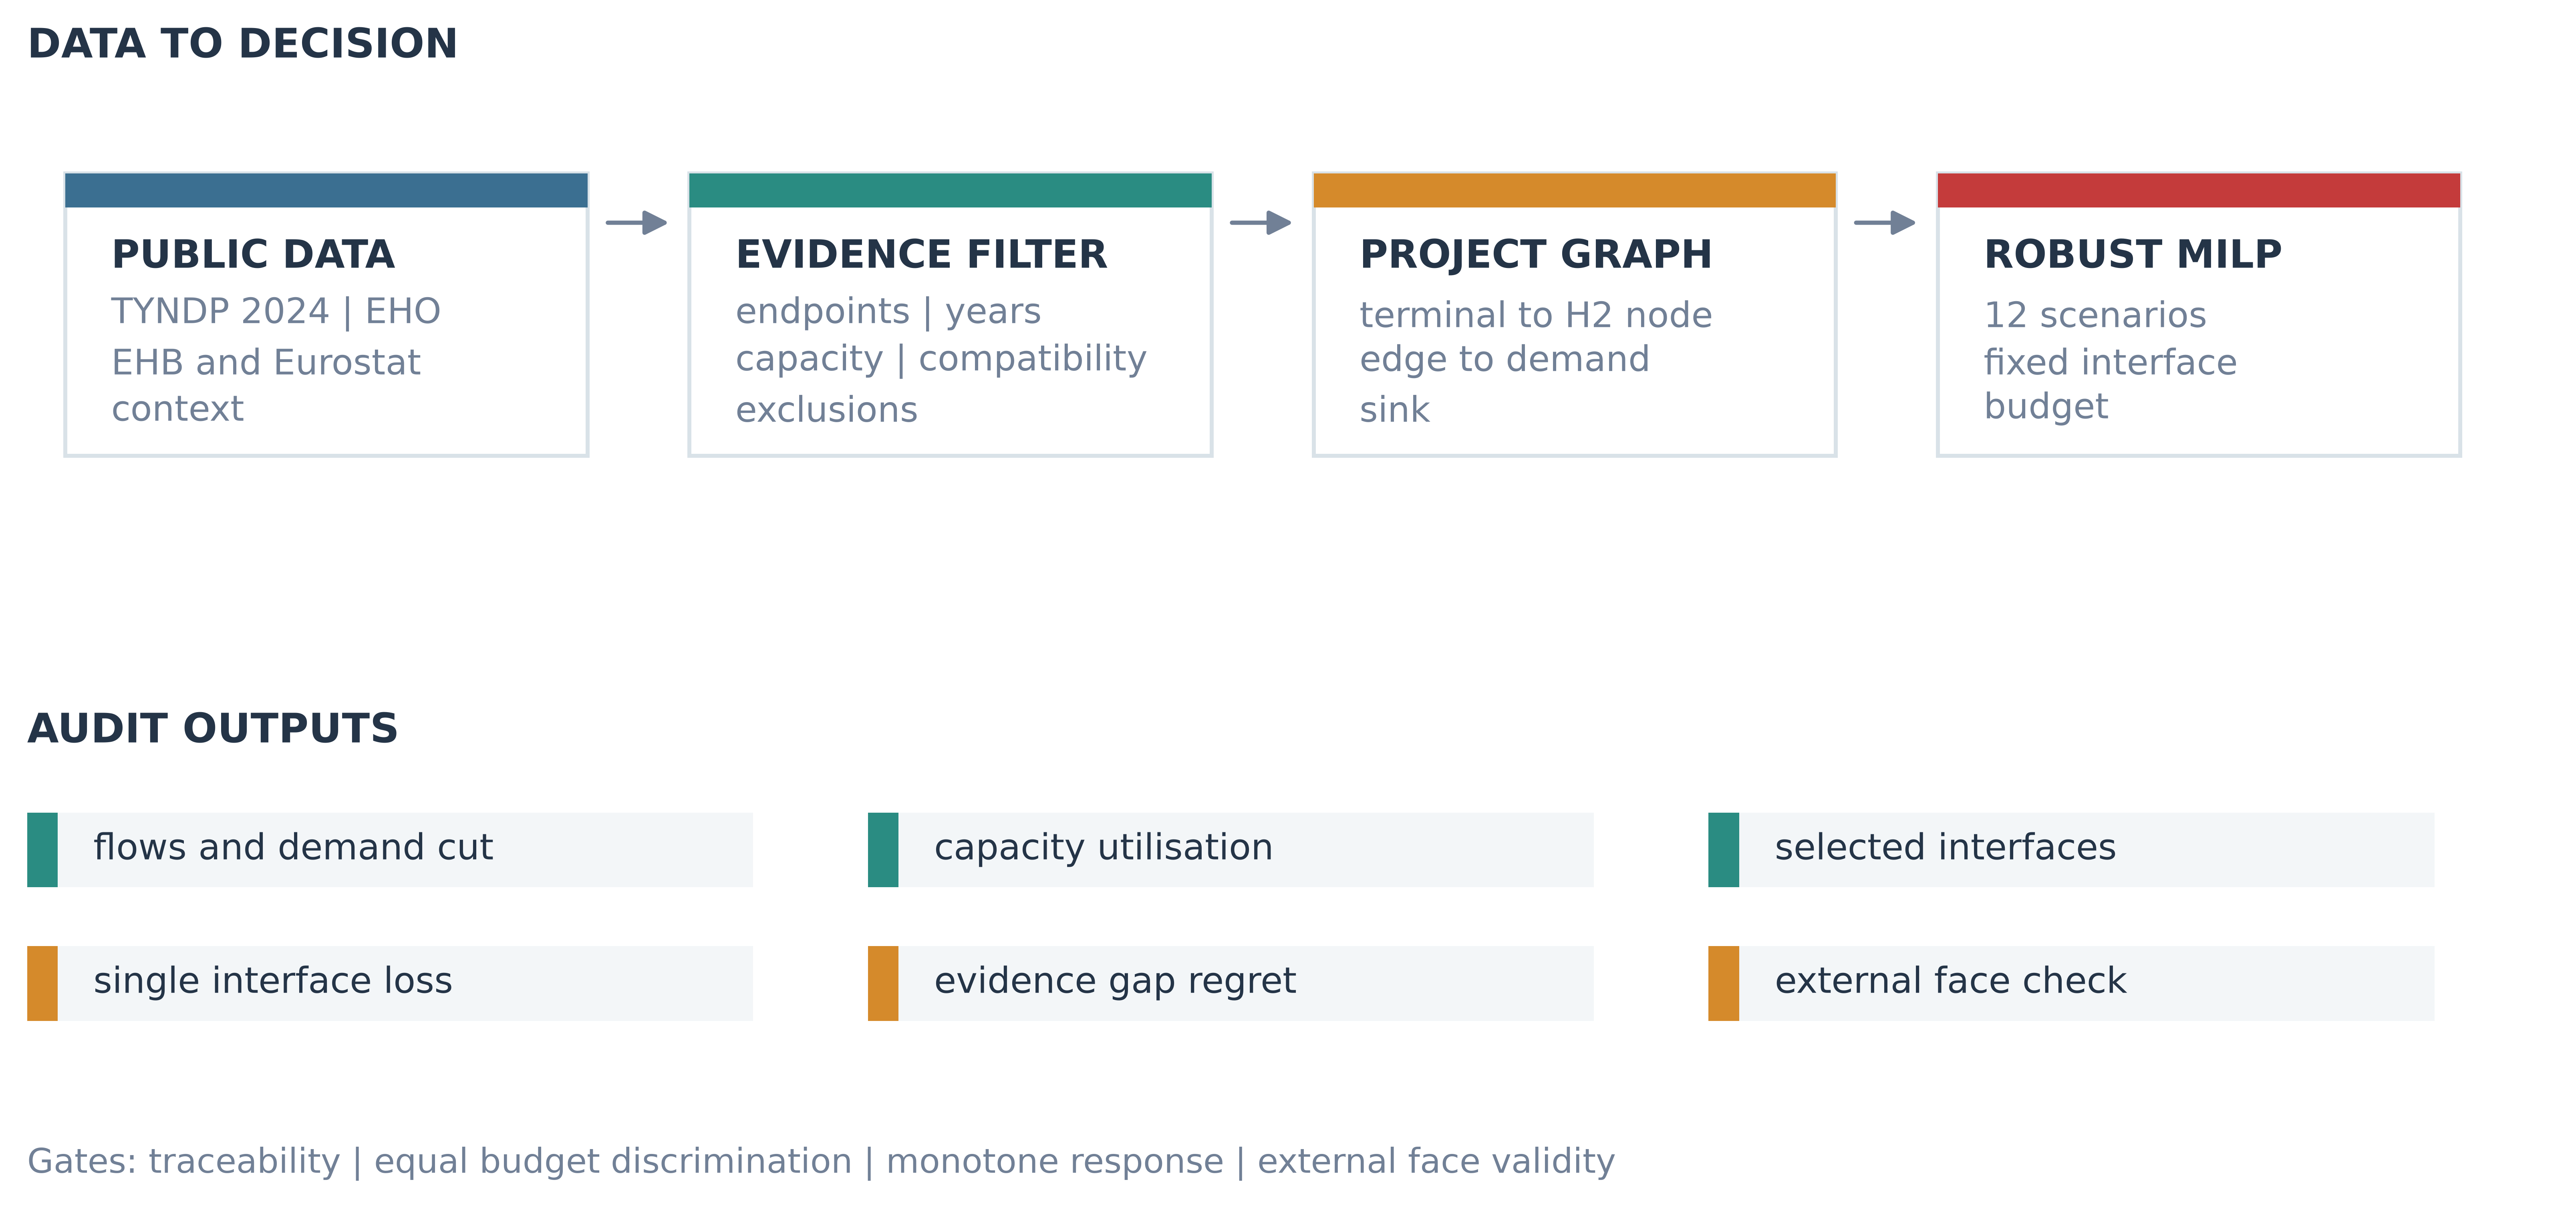
\includegraphics[width=0.98\textwidth]{figure1_data_lineage.png}
\caption{Audit workflow from public records to the priority verification set. The upper sequence shows data filtering, graph construction, and scenario based robust selection. The lower strip lists the observable outputs and diagnostic gates.}
\label{fig:lineage}
\end{figure*}

\begin{figure*}[t]
\centering
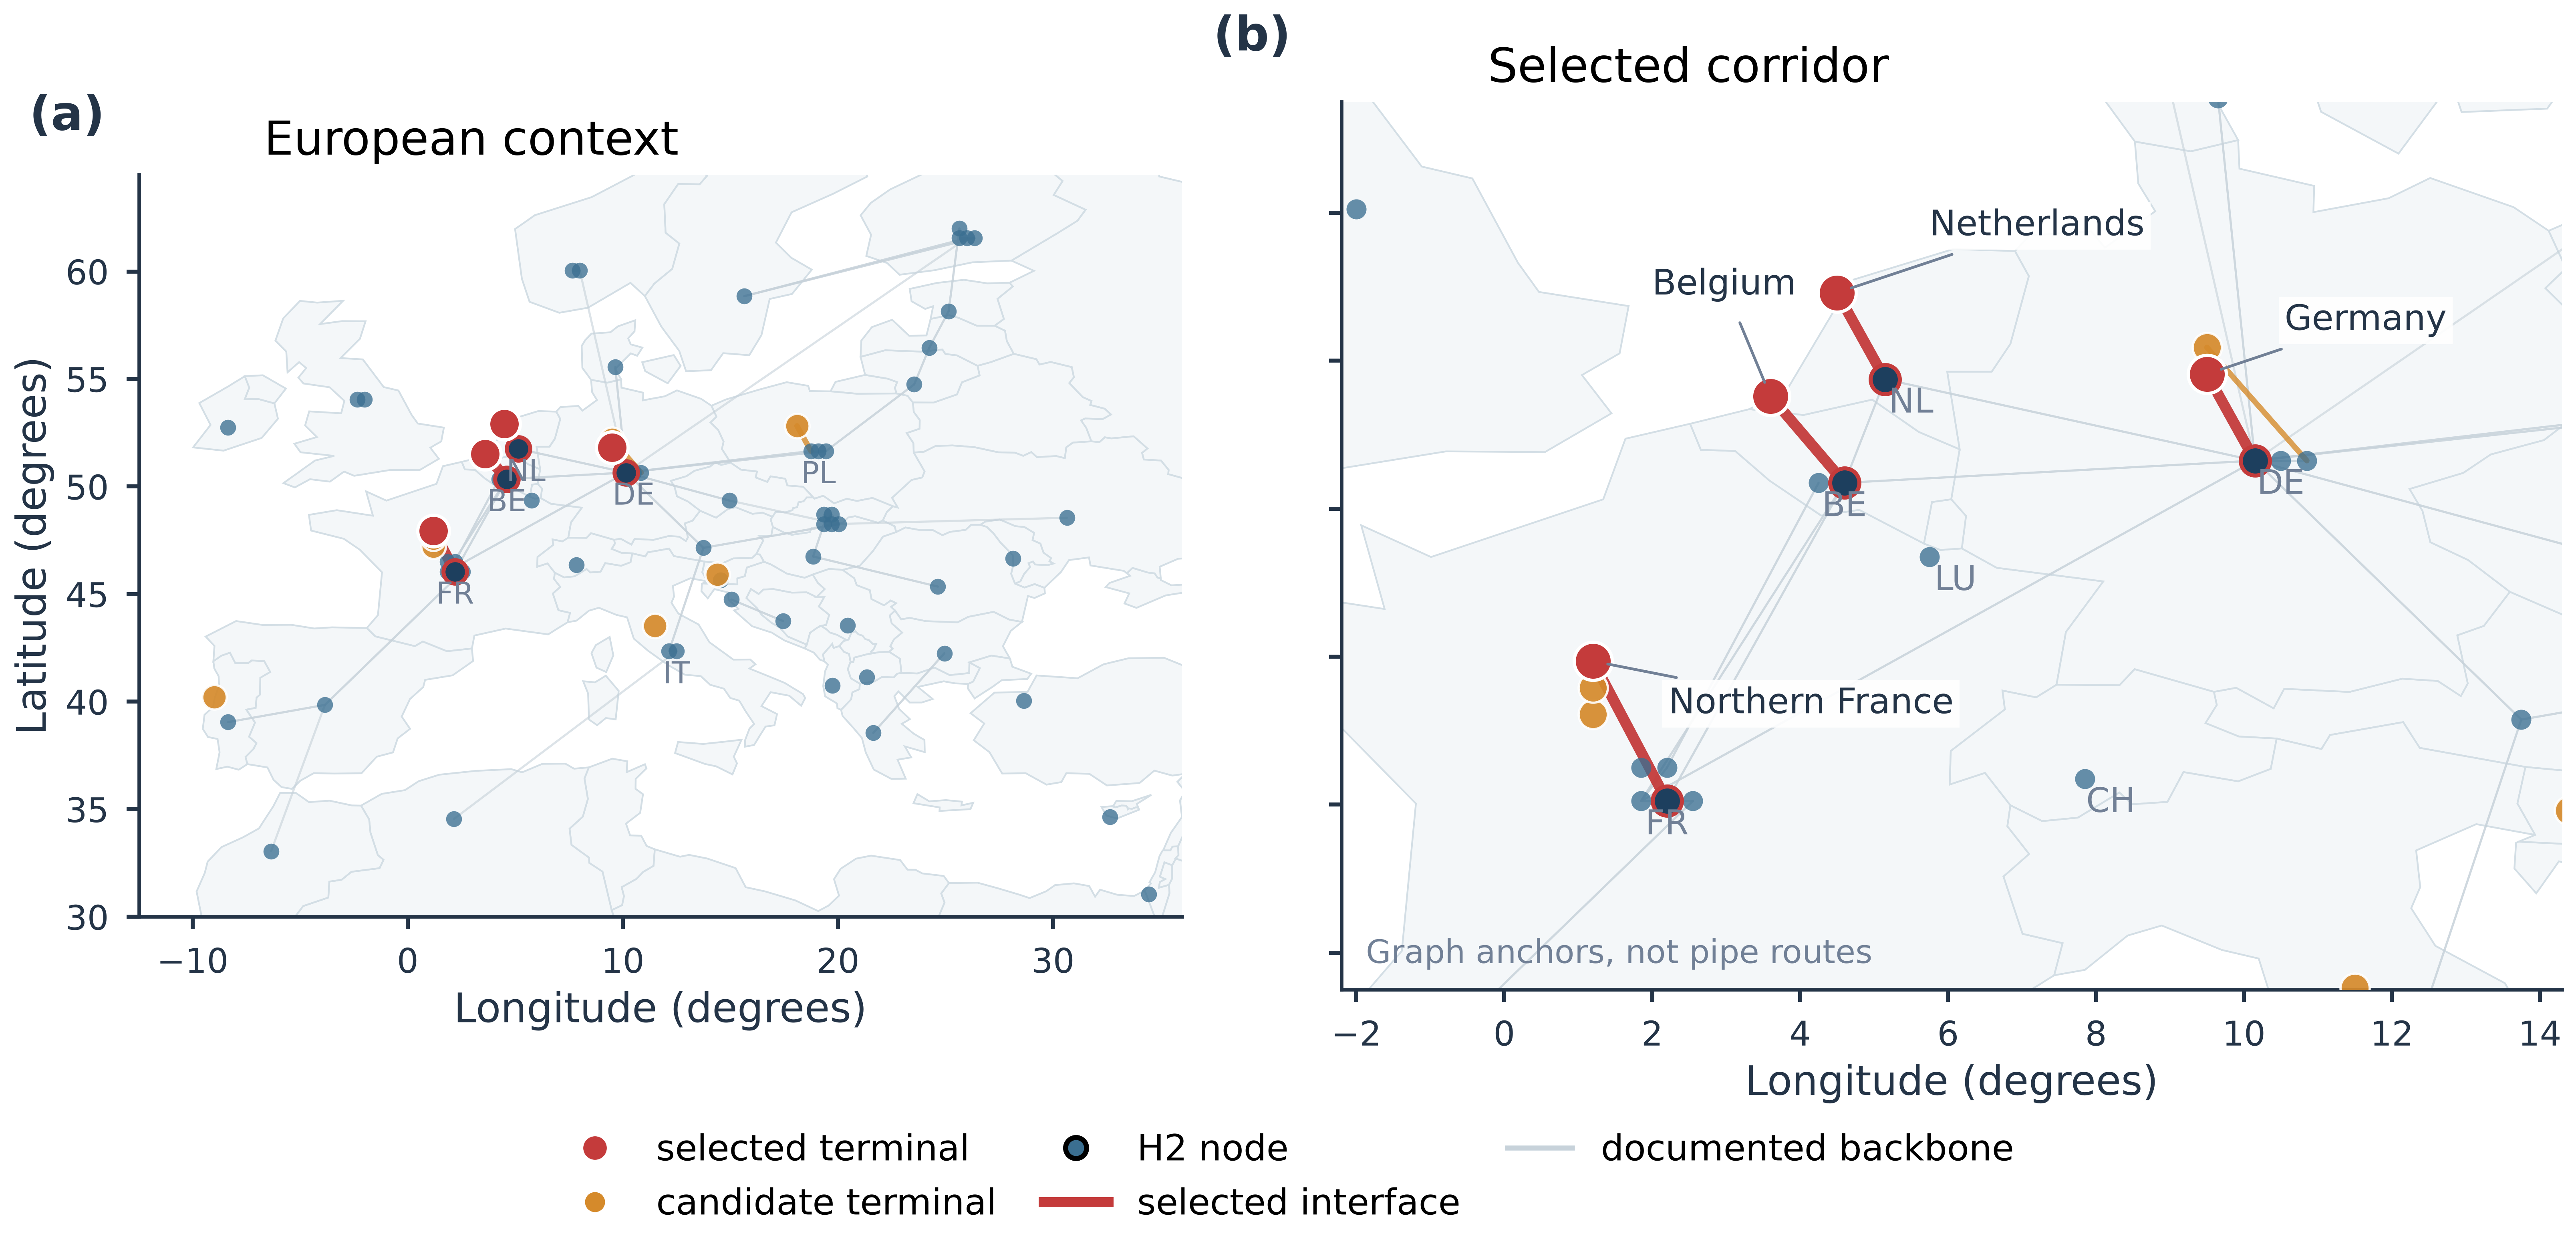
\includegraphics[width=0.98\textwidth]{figure2_project_graph.png}
\caption{Project graph view of modeled terminal and backbone interfaces. (a) European context. (b) Enlarged view of the selected corridor. Red links mark the four interfaces selected for priority verification, orange marks other candidate terminal connections, and pale links show documented backbone adjacency. Light grey country outlines use the Natural Earth 1:110m visualization asset \cite{NaturalEarth}. Country anchors provide geographic context only; graph links are not geographic pipe geometries.}
\label{fig:graph}
\end{figure*}

Figure~\ref{fig:graph} shows the modeled terminal and backbone interfaces in their geographic context. Panel (a) provides the European reference frame, and panel (b) enlarges the four selected groups. The selected red links identify the priority verification groups, while pale links retain the documented backbone adjacency. Country outlines and anchors provide orientation; the links depict graph adjacency, while physical pipeline geometry requires separate spatial evidence.

\subsection{Carrier compatibility and direct ammonia boundary}

The core service variable is hydrogen equivalent energy entering the backbone. Liquid hydrogen and converted carrier routes can therefore serve hydrogen demand after the relevant terminal and conversion evidence is admitted. Direct \NHthree{} is reserved for a separate sensitivity because the EHO category labelled "ammonia" describes hydrogen feedstock demand without verifying direct NH3 consumption at a named sink. The unchanged counterfactual result confirms that the main portfolio is stable under this eligibility boundary.

\subsection{Interpretation of planning records}

The public product supplies planning records: TYNDP capacities and project statuses, EHO facility coordinates and demand envelopes, and explicit terminal and backbone records. These records support an annual capacity screen and an evidence prioritization result. Operational throughput, berth queues, storage inventories, hourly utilization, facility level conversion yields, firm contracts, capital expenditure, and project finance form the next evidence layer. Accordingly, the model output is a verification priority and scenario stress metric under the stated scope, suitable for front end engineering screening.

\section{Two Stage Lexicographic Scenario Based Robust MILP}
\label{sec:model}

\subsection{Sets and variables}

Let $\mathcal{S}$ be the 12 design scenarios, $\mathcal{N}$ the graph nodes, $\mathcal{E}$ the directed backbone edges, $\mathcal{T}$ the terminal interface candidates, $\mathcal{K}$ the carrier classes, and $\mathcal{F}$ the facilities. A scenario $s$ is defined by a horizon $h\in\{2030,2040\}$, an infrastructure level $\ell\in\{\mathrm{PCI/PMI},\mathrm{Advanced}\}$, and a demand level $d\in\{\mathrm{low},\mathrm{medium},\mathrm{high}\}$.

This paper uses the term scenario based robust screening for minimax selection over the fixed 12 scenario set. The scenario matrix is declared before optimization, and the first stage minimizes the worst unmet demand ratio across that finite set. This finite scenario formulation is distinct from continuous robust optimization with ellipsoidal or polyhedral uncertainty sets, which would require additional distributional information. The distinction defines the interpretation of the reported MILP.

Binary variables $y_{tk}$ and $z_t$ indicate that a terminal and carrier or terminal and backbone interface is in the priority verification set. Under the stated scope, these variables allocate verification priority; construction, permitting, ownership, and investment decisions belong to subsequent engineering stages. Scenario recourse variables are nonnegative carrier injections $q_{tks}$, backbone flows $f_{es}$, facility service $v_{is}$, and unmet demand $u_{is}$.

\subsection{Design rationale}

Three engineering rules determine the formulation. First, the interface budget is fixed at four because the practical bottleneck is verification capacity: a port or network team must be able to follow each selected record into a named terminal, project, capacity, and status file. The budget is a screening resource constraint, while construction budgets require a separate investment model. Second, carrier records without a terminal crosswalk remain in shared country and carrier pools. This avoids counting one project announcement at multiple terminals while still allowing the record to inform country level availability. Third, the first stage set is selected against the complete declared scenario matrix, and the recourse allocation is solved after each set is fixed. A lexicographic objective then prioritizes the worst scenario, the total unmet amount, and finally the number of activated interface flags.

\subsection{Flow balance and capacity}

For every scenario, flow conservation is imposed on network nodes that can receive flow from a terminal and on all backbone transshipment nodes:
\begin{equation}
\sum_{e\in\delta^-(n)}f_{es}+\sum_{t,k:n(t)=n}q_{tks}
-\sum_{e\in\delta^+(n)}f_{es}=0.
\label{eq:flow}
\end{equation}
Equation~\eqref{eq:flow} prevents flow creation or loss at modeled network nodes.

At a facility, service and unmet demand sum to the scenario demand:
\begin{equation}
v_{is}+u_{is}=D_{is},\qquad i\in\mathcal{F},\ s\in\mathcal{S}.
\label{eq:demand}
\end{equation}
Equation~\eqref{eq:demand} separates served demand from unmet demand for every facility and scenario.

For each directed edge $e$:
\begin{equation}
0\leq f_{es}\leq C_{es},\qquad e\in\mathcal{E},\ s\in\mathcal{S},
\label{eq:edge-capacity}
\end{equation}
The edge capacity restriction in \eqref{eq:edge-capacity} is evaluated separately for each planning scenario.
where $C_{es}$ is read from the frozen year, status, and infrastructure level fields. A terminal interface is gated by the corresponding first stage verification binary:
\begin{equation}
q_{tks}\leq C^{\mathrm{term}}_{ts}z_t,\qquad
q_{tks}\leq P_{cks}y_{tk}.
\label{eq:interface}
\end{equation}
The two inequalities in \eqref{eq:interface} require both a selected interface and an available carrier pool before a terminal injection is admitted.
Here $P_{cks}$ is a shared country and carrier pool. For every country $c$ and carrier $k$:
\begin{equation}
\sum_{t\in\mathcal{T}_c}q_{tks}\leq P_{cks}.
\label{eq:pool}
\end{equation}
The shared-pool constraint in \eqref{eq:pool} prevents the same project record from being counted at multiple terminals.
The shared pool prevents one anonymous project record from being counted repeatedly at several terminal nodes.

\subsection{Lexicographic objective and fixed budget}

Define $U_s=\sum_i u_{is}$ and $D_s=\sum_iD_{is}$. The first stage and recourse problem is solved with the lexicographic objective
\begin{equation}
\min\ \operatorname{lex}\left(
\max_{s\in\mathcal{S}}\frac{U_s}{D_s},
\sum_{s\in\mathcal{S}}U_s,
\sum_{t,k}y_{tk}+\sum_tz_t
\right).
\label{eq:objective}
\end{equation}
The lexicographic objective in \eqref{eq:objective} ranks portfolios by worst scenario first, aggregate unmet demand second, and interface flags third.
An epigraph variable represents the first component. The lexicographic construction uses unmet demand directly rather than an arbitrary penalty weight. The reported main selection uses a fixed interface budget of four unique terminal and backbone candidates, with carrier variables activated consistently with the selected terminal groups. The deterministic comparator selects its four candidates in the central planning scenario and is then evaluated over the same 12 scenarios. The scenario based robust and deterministic formulations produce the same selection in this frozen data product. This equality is reported as an empirical boundary, while the evidence ablations and failure diagnostics test whether the workflow remains useful beyond the central scenario.

\subsection{Failure stress recourse}

The N--1 and N--2 tests are conducted after first stage selection. In an N--1 run, one selected interface is removed from the available graph and the fixed four interface portfolio is re evaluated. N--2 removes each pair of selected interfaces. The failure tests therefore examine the exposure of the verification set without allowing the first stage selector to adapt after observing the failure. They provide failure stress diagnostics under the interpretation boundary stated above.

\section{Experimental Protocol and Predefined Gates}
\label{sec:protocol}

\subsection{Core scenarios}

The planning matrix is frozen as 2030/2040 $\times$ PCI/PMI or Advanced $\times$ low/medium/high EHO demand, giving 12 scenarios. The eight TYNDP Hydrogen import cases are reserved for an external corridor face check. No model parameter is tuned to match that external file after observing the comparison.

\subsection{Comparators and ablations}

The same data and demand envelope are run through five structural specifications:
\begin{enumerate}
\item a topology free port and country star LP;
\item a project graph LP without carrier compatibility;
\item a project graph LP with carrier compatibility and shared pools;
\item an equal budget deterministic MILP; and
\item the proposed equal budget scenario based robust MILP.
\end{enumerate}
The star model is an intentionally permissive upper bound comparator whose deleted path and interface restrictions distinguish it from the project graph. The exact equal budget comparator enumerates all $\binom{9}{4}=126$ portfolios and evaluates each portfolio over the 12 planning scenarios. The exact census is the primary comparison; fixed seed random draws are reported separately as a distributional sanity check.

\subsection{Predefined success gates}

Table~\ref{tab:gates} lists the preregistered engineering gates, their thresholds, and the observed outcomes. The gates test traceability, portfolio separation, evidence gap detectability, failure stress behavior, capacity monotonicity, and external corridor overlap.

\begin{table*}[t]
\centering
\caption{Preregistered engineering gates and observed outcomes}
\label{tab:gates}
\scriptsize
\begin{tabularx}{\textwidth}{p{3.4cm}p{4.5cm}Xc}
\toprule
Gate & Threshold & Observed result & Pass \\
\midrule
Traceability & 100\% of included corridor inputs & All frozen corridor inputs traceable & Yes \\
Portfolio discrimination & Scenario robust worst \DCR{} at least 5 percentage points below random median and below random 90th percentile & 22.179 and 44.284 percentage point gains & Yes \\
Evidence gap detection & At least 1 percentage point regret after an evidence ablation & Maximum regret 22.105 percentage points & Yes \\
N--1 noninferiority & Scenario robust worst \DCR{} no greater than deterministic worst \DCR{} & 77.895\% versus 77.895\% & Yes \\
Capacity response & Higher capacity multiplier cannot increase worst \DCR{} & 77.858\%, 55.716\%, 33.574\% at 0.5, 1.0, 1.5 & Yes \\
External corridor face & At least two of four top countries selected in 2030 and 2040 & Overlap 2 in both years & Yes \\
\bottomrule
\end{tabularx}
\end{table*}

All six gates in Table~\ref{tab:gates} pass for the frozen product. They establish the evidence and scenario conditions under which the reported screening result should be read, while preserving the stress metrics as screening quantities.

The IGI indicators are retained as a construct comparison rather than a pass or fail gate. IGI hotspot rankings and this paper's interface priority ranking are generated for different objects, so a direct replication threshold would conflate infrastructure gap identification with terminal interface screening. The comparison remains useful for reporting where the two constructs overlap and where they diverge.

\section{Results}
\label{sec:results}

\subsection{Equal budget portfolio census}

The first result is an exact comparison over all $\binom{9}{4}=126$ four interface portfolios. The selected portfolio has the minimum observed worst planning \DCR{} of 55.72\%. The portfolio distribution has a median of 77.89\%, a mean of 80.32\%, and a 90th percentile of 100\%. Thus, the screen improves on the equal budget median and 90th percentile by 22.18 and 44.28 percentage points, respectively. The minimum equals the MILP result, so the evidence supports a best observed portfolio within the audited candidate set and verification budget.

Figure~\ref{fig:portfolio} displays the complete equal budget distribution and the corresponding separation from the selected portfolio. Panel (a) places the selected value at the lower tail of the 126 portfolio distribution. Panel (b) reports the observed separation from the median and 90th percentile; these are census comparisons, not statistical significance tests.

\begin{figure*}[t]
\centering
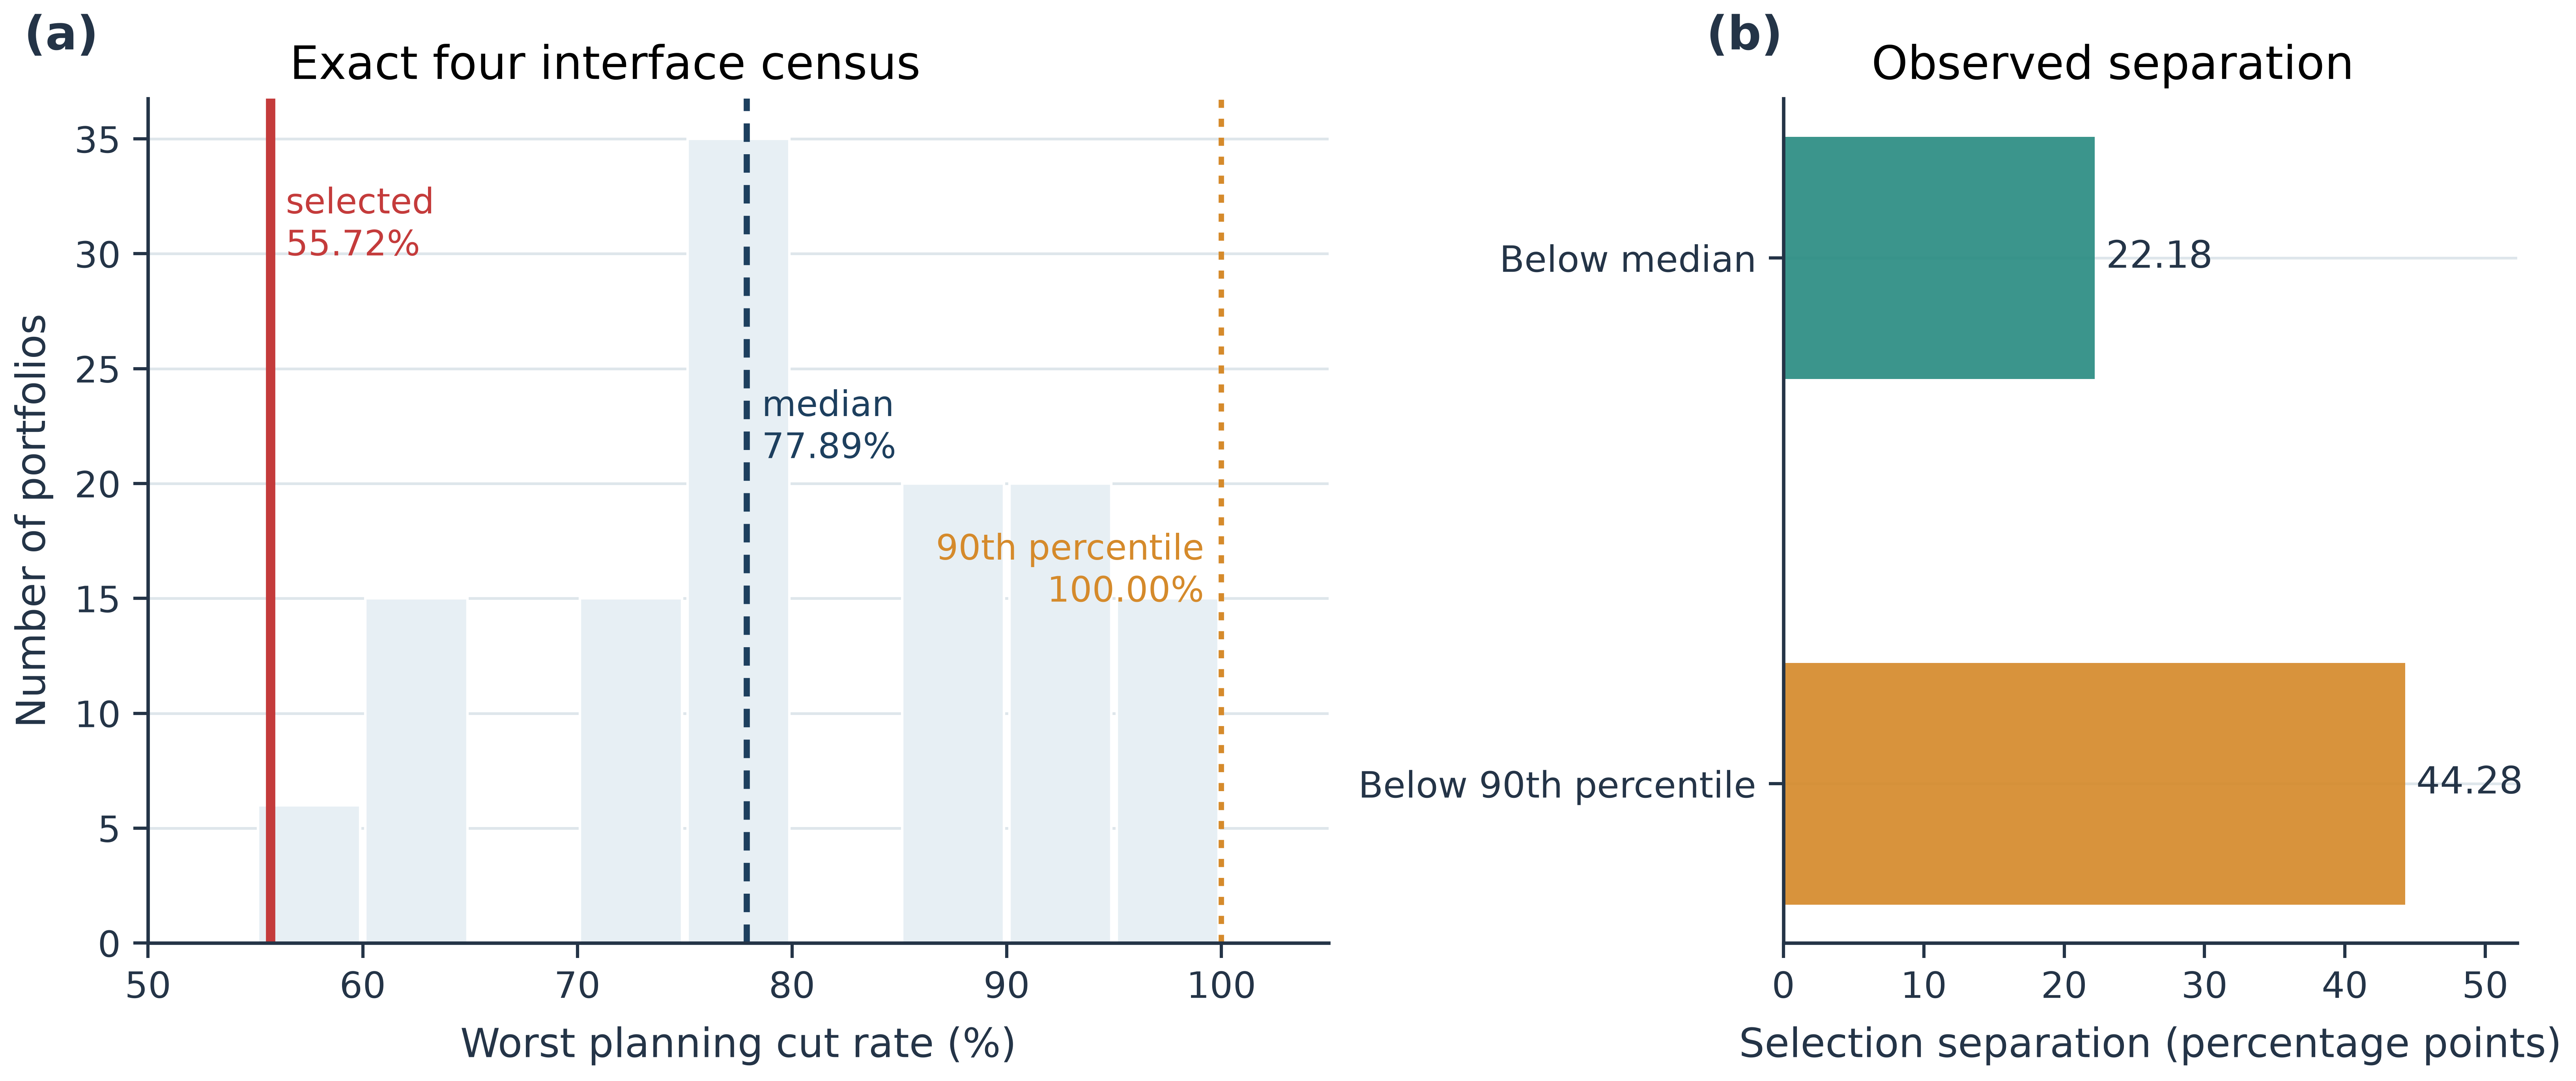
\includegraphics[width=0.98\textwidth]{figure3_portfolio_vs_random.png}
\caption{Exact equal budget portfolio census. (a) Distribution of worst planning cut rates across 126 four interface portfolios, with the selected portfolio, median, and 90th percentile marked directly. (b) Separation of the selected portfolio from the two reference quantiles.}
\label{fig:portfolio}
\end{figure*}

\subsection{Evidence gap regret}

The second result translates the portfolio comparison into a data collection priority. Removing explicit capacity evidence changes the N--1 failure stress from 77.89\% to 100\%, an increase of 22.11 percentage points in planning stress when that evidence layer is unavailable. Removing carrier evidence or omitting the demand uncertainty layer leaves the selected set unchanged in this frozen product. Capacity documentation is therefore the dominant evidence collection priority in the present screen, while the null ablations identify inputs whose current records do not change the portfolio.

Figure~\ref{fig:evidence-gap} compares the failure stress change after each evidence layer is withheld. Panel (a) shows the 22.11 percentage point stress shift when capacity evidence is removed. Panel (b) attributes the shift to the capacity ablation, while carrier and demand ablations remain at zero in the frozen product. The figure identifies the next evidence layer to verify, not the economic value of a project.

The engineering implication is direct: capacity evidence should be collected first. The relevant check is whether the interface and its backbone connection have a documented and traceable capacity. The metric orders evidence collection; economic valuation belongs to a separate project appraisal.

The direct ammonia boundary sensitivity also passes. Varying the direct NH3 service share from 0\% to 50\% and 100\% leaves the selected portfolio unchanged and retains a 55.716\% worst curtailment rate, a 21.513\% mean rate, and 358,030 GWh of unmet demand. The main selection is therefore stable under the tested ammonia eligibility boundary.

\begin{figure*}[t]
\centering
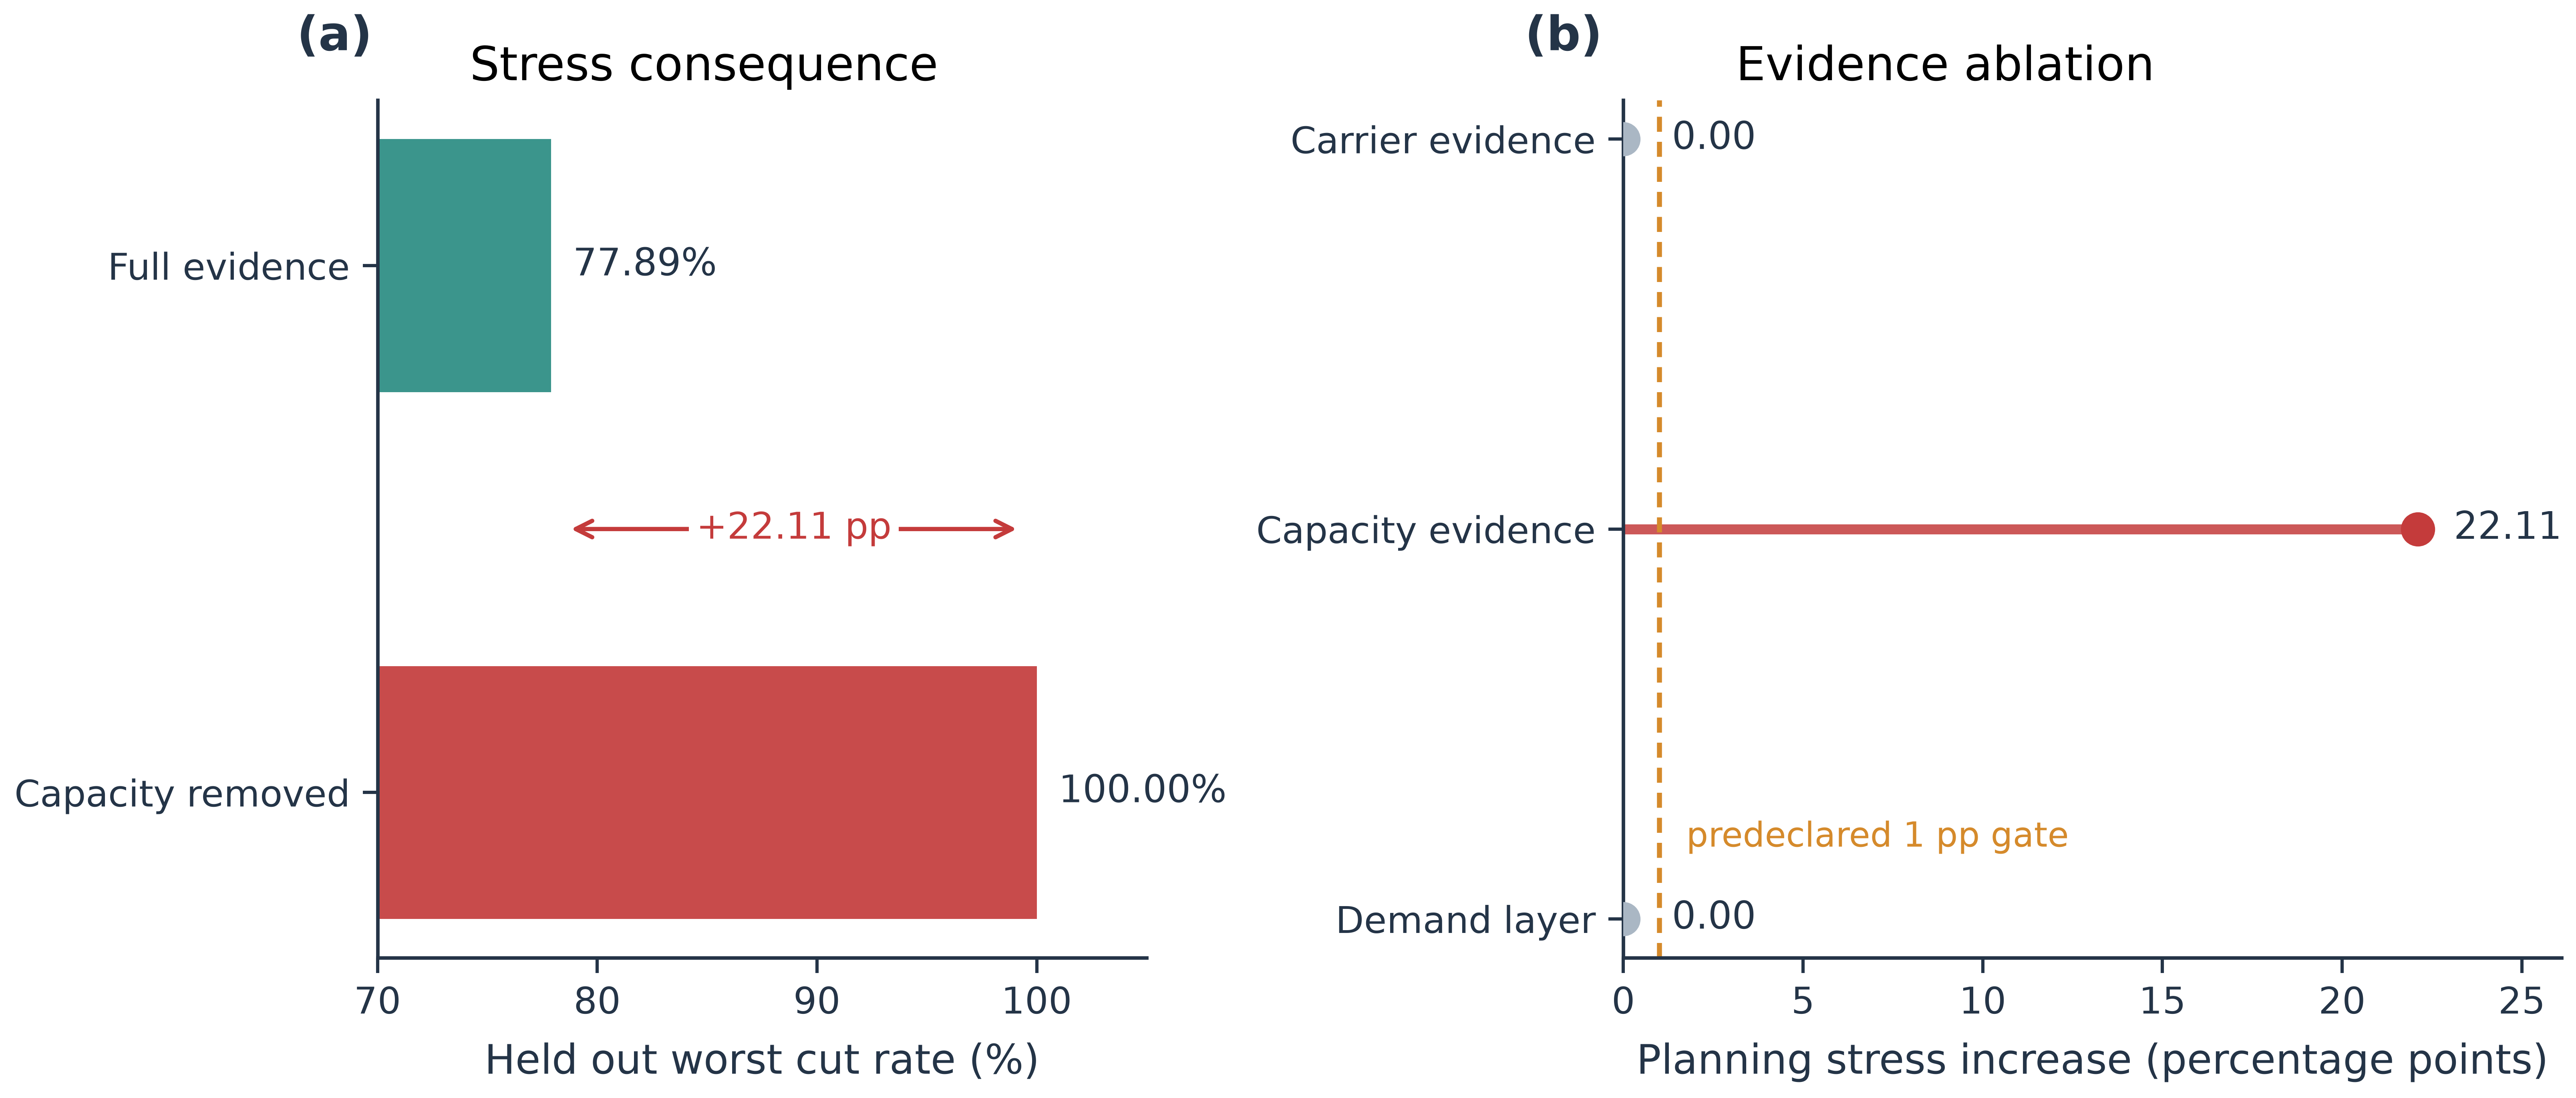
\includegraphics[width=0.98\textwidth]{figure4_data_gap_regret.png}
\caption{Evidence gap diagnosis. (a) N--1 failure stress with the full evidence product and after capacity evidence is removed. (b) Increase in planning stress for each withheld evidence layer, measured in percentage points of N--1 worst curtailment.}
\label{fig:evidence-gap}
\end{figure*}

\subsection{Selected verification set and base performance}

The scenario based robust selector returns four interface groups: the Belgium terminal to the Belgium hydrogen node, the Germany terminal to the Germany hydrogen node, the northern France terminal to the northern France hydrogen node, and the Netherlands terminal to the Netherlands hydrogen node. These names identify modeled endpoint relationships for verification priority; construction decisions and physical route design require the subsequent engineering evidence layer.
The deterministic central scenario selector returns the same set. Across the 12 planning scenarios, the selected portfolio has a mean demand curtailment rate of 21.51\%, a worst rate of 55.72\%, and total unmet demand of 358,030 GWh. The worst case occurs in the 2030 PCI/PMI high demand scenario. The four interface set is not presented as a geographic discovery; its engineering value is the exact portfolio census and the evidence gap ranking.

Table~\ref{tab:priority} reports the selected interfaces, their modeled demand curtailment statistics, and their N--1 failure effects. The Netherlands interface has the largest single interface effect, while northern France has no additional worst rate effect in the tested scenario matrix.

\begin{table}[t]
\centering
\caption{Selected interface priority and N--1 criticality}
\label{tab:priority}
\scriptsize
\setlength{\tabcolsep}{2.5pt}
\begin{tabular}{@{}lrrrr@{}}
\toprule
Interface & Mean & Max & N--1 & Delta \\
\midrule
Belgium & 94.19\% & 100\% & 70.20\% & 14.48 pp \\
Germany & 100.00\% & 100\% & 63.34\% & 7.62 pp \\
N. France & 100.00\% & 100\% & 55.72\% & 0.00 pp \\
Netherlands & 97.22\% & 100\% & 77.89\% & 22.18 pp \\
\bottomrule
\end{tabular}
\end{table}

Table~\ref{tab:priority} distinguishes verification urgency from modeled volume. Its utilization columns are modeled capacity ratios that provide a consistent basis for screening comparisons.

For verification planning, the Netherlands interface has the largest single interface effect at 22.18 percentage points. It is therefore the first candidate when one verification resource must be allocated to reduce worst case stress. This priority is relative to the current candidate set. Northern France has zero incremental worst rate effect in the current matrix, although it still changes scenario specific flows and merits additional evidence review.

\subsection{Structural ablation and carrier boundary}

Table~\ref{tab:ablation} compares the topology free star LP, the two project graph LP variants, and the deterministic and scenario based robust MILP selectors. The table separates the effect of network topology from the effect of carrier compatibility and scenario selection.

\begin{table*}[t]
\centering
\caption{Structural ablation over the 12 planning scenarios}
\label{tab:ablation}
\scriptsize
\begin{tabularx}{\textwidth}{p{4.2cm}rrrX}
\toprule
Specification & Worst \DCR{} (\%) & Mean \DCR{} (\%) & Unmet demand (GWh) & Interpretation \\
\midrule
Port and country star LP & 52.54 & 17.09 & 285,442 & Topology free upper bound diagnostic. \\
Project graph LP, generic carrier & 55.72 & 18.50 & 309,167 & Network topology admitted. \\
Project graph LP, compatible carrier & 55.72 & 18.50 & 309,167 & Shared carrier pools added. \\
Deterministic four interface MILP & 55.72 & 21.51 & 358,030 & Central scenario selection. \\
Scenario robust four interface MILP & 55.72 & 21.51 & 358,030 & Joint scenario selection. \\
\bottomrule
\end{tabularx}
\end{table*}

The ablation shows why topology and shared pools belong in the engineering screen. Removing topology makes the system appear less constrained by deleting path and interface restrictions. Carrier compatibility does not change this aggregate result because the binding bottleneck is the admitted interface and backbone capacity rather than the carrier label. In the present product, carrier compatibility therefore functions as a feasibility safeguard, while the selected portfolio is governed by the admitted interface and backbone capacities.

Figure~\ref{fig:ablation} presents the same comparison visually. The star LP has the lowest apparent worst curtailment because it removes path and interface restrictions, whereas the graph based specifications converge at 55.72\%. The visual result supports the use of the project graph as a conservative engineering screen.

\begin{figure*}[t]
\centering
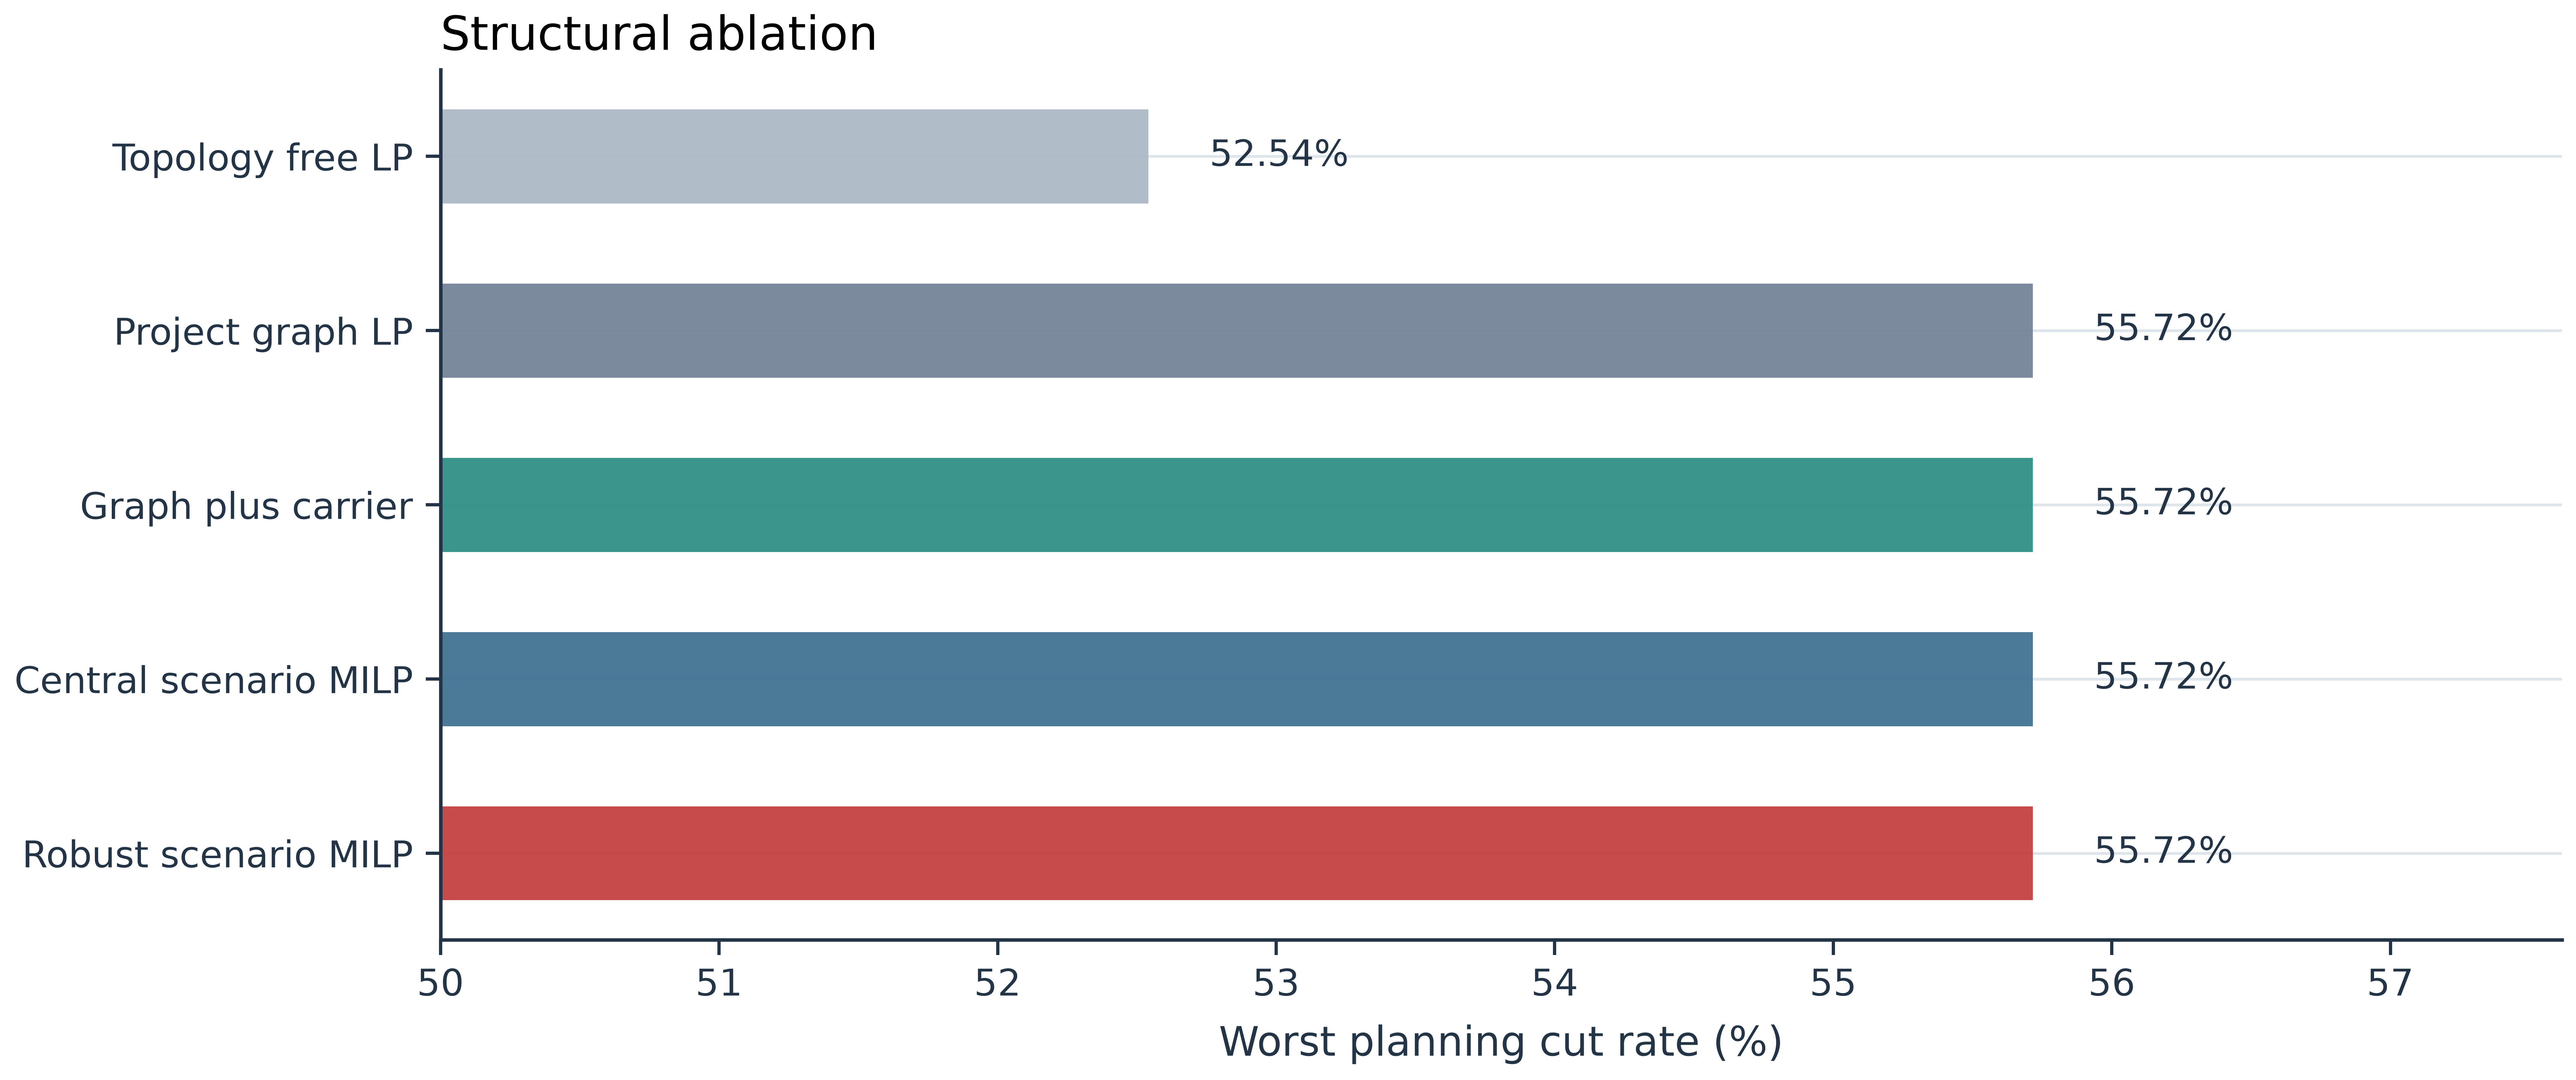
\includegraphics[width=0.98\textwidth]{figure3_structural_ablation.png}
\caption{Structural ablation of the corridor screen. Topology and shared capacity pools prevent an optimistic upper bound from being interpreted as a feasible interface screen.}
\label{fig:ablation}
\end{figure*}

\subsection{Interface failure stress analysis}

Under N--1 failure of the selected four interfaces, the worst curtailment is 77.89\%. The Netherlands interface is the most critical individual failure, increasing the worst rate by 22.18 percentage points; Belgium increases it by 14.48 points and Germany by 7.62 points. Removing northern France does not increase the worst planning rate in the tested matrix, although it changes scenario specific flows. This ranking orders contingency evidence priorities; failure probability estimation requires a separate reliability data product.

The worst N--2 result is 92.38\%. The N--1 result passes the predefined noninferiority gate because the scenario based robust and deterministic selections are identical. In this frozen case, the result establishes parity rather than a numerical advantage of scenario based robust selection over deterministic selection.

Figure~\ref{fig:resilience} reports the N--1 failure effect for each selected interface and the N--2 envelope. The Netherlands interface produces the largest individual increase, followed by Belgium and Germany, while northern France has no additional worst rate effect in this matrix. These values prioritize contingency evidence; probability estimates require a separate reliability data product.

\begin{figure*}[t]
\centering
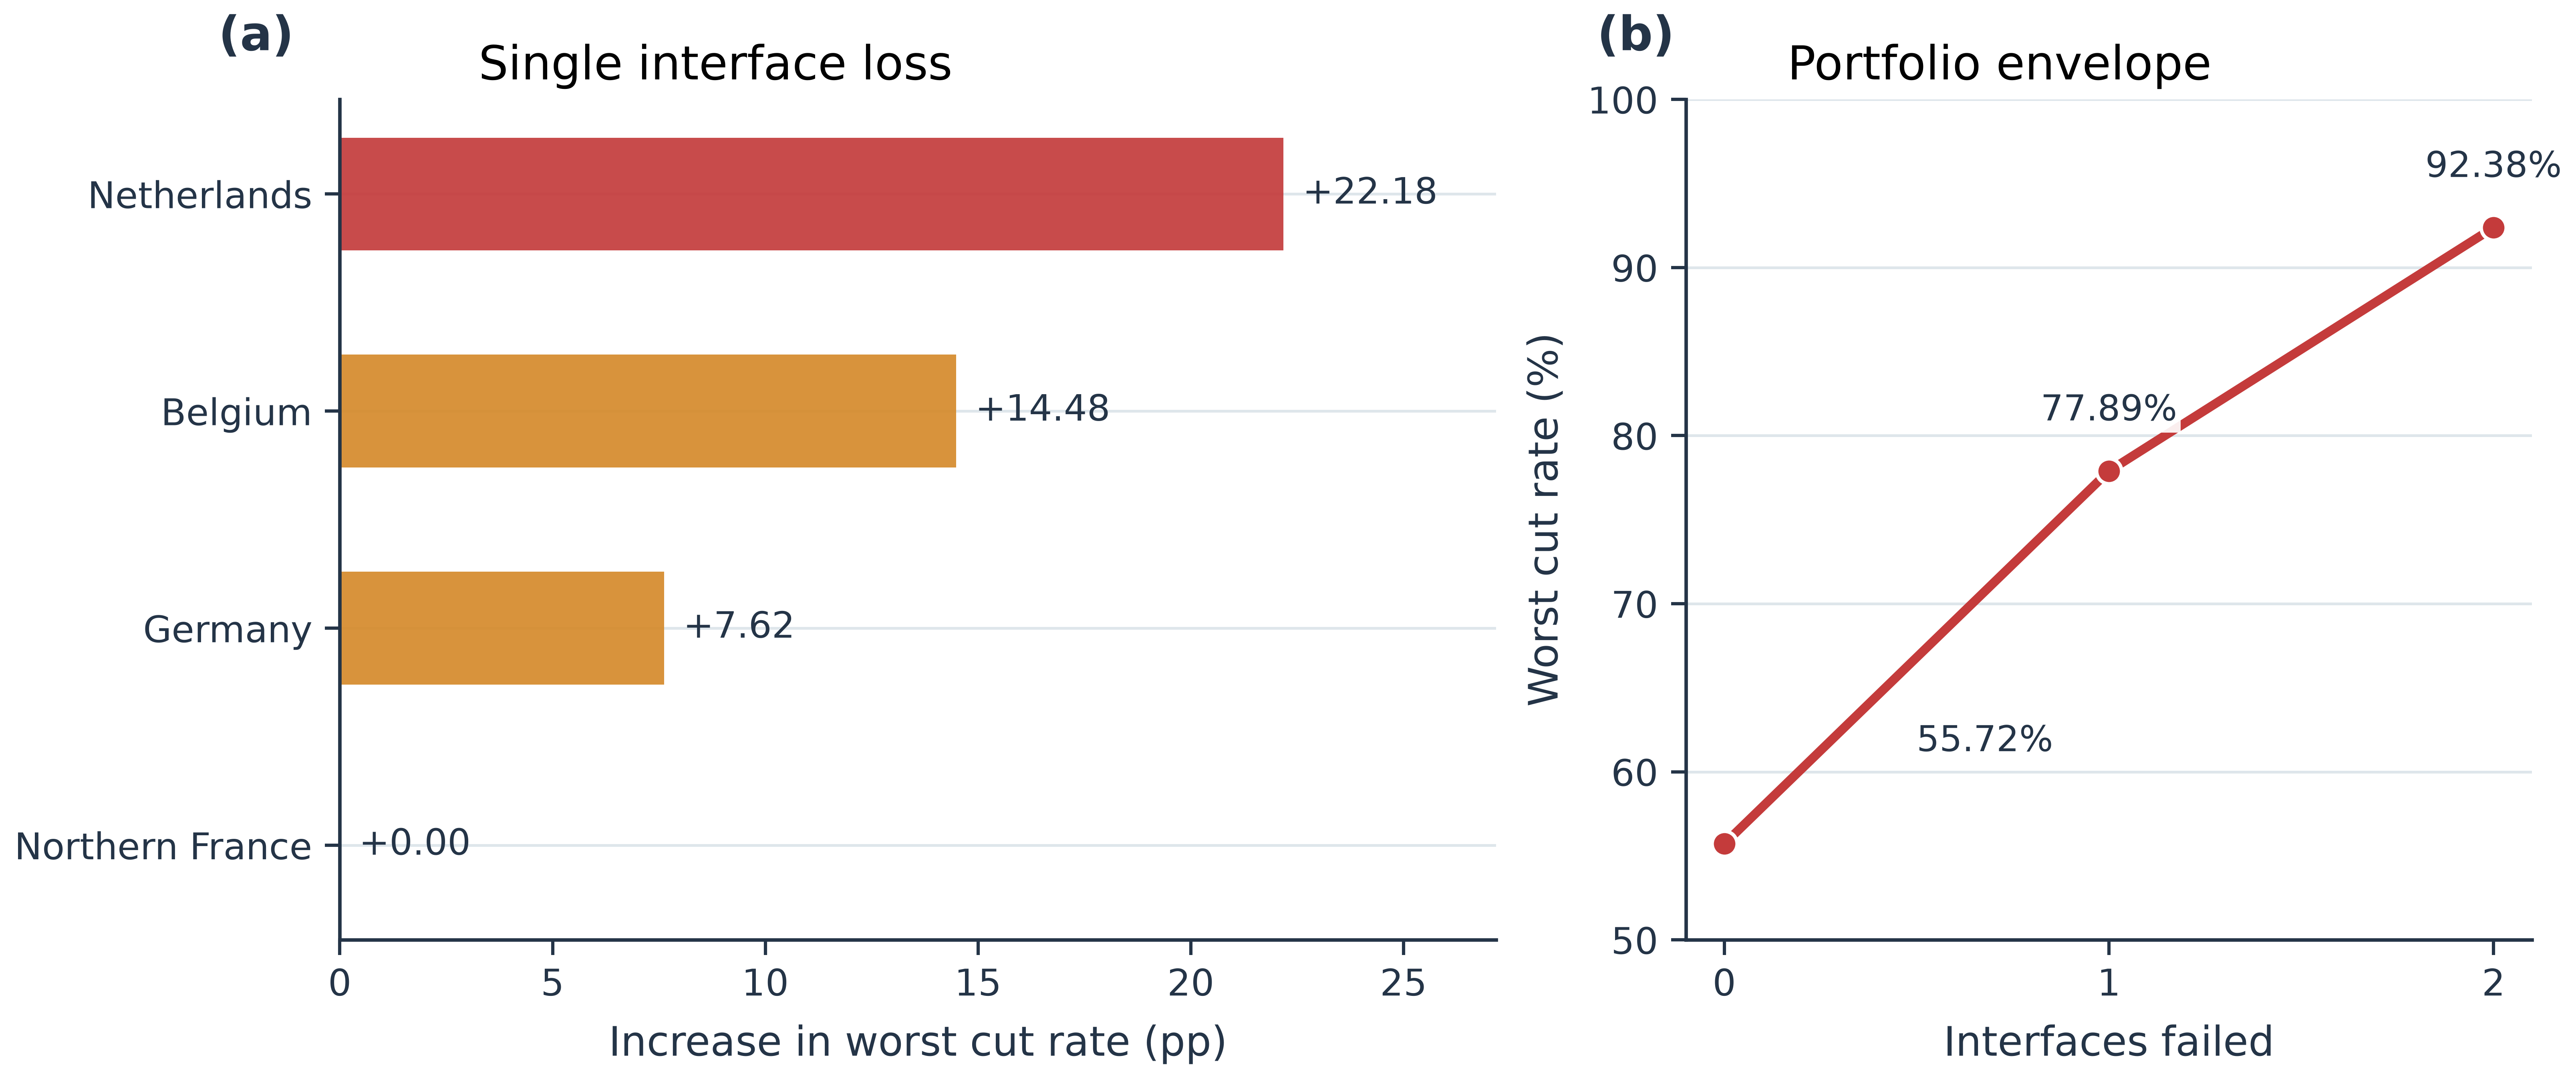
\includegraphics[width=0.98\textwidth]{figure5_nk_resilience.png}
\caption{Interface failure stress diagnostics. (a) Increase in worst cut rate after removal of each selected interface. (b) Worst cut rate as one or two selected interfaces are removed simultaneously.}
\label{fig:resilience}
\end{figure*}

\subsection{Capacity and external corridor sensitivity}

Scaling all modeled backbone and terminal capacities by 0.5, 1.0, and 1.5 gives worst planning curtailment rates of 77.86\%, 55.72\%, and 33.57\%, respectively. The monotone response is an internal consistency check: capacity relaxation does not make the screen worse.

The external TYNDP Hydrogen import generator file is used for a face validity check, with no calibration step. The four selected countries overlap two of the external top four in 2030 and two in 2040. Weighted coverage is 62.80\% in 2030 and 46.66\% in 2040. The partial overlap is the appropriate interpretation: the two products share a corridor object but have different aggregation and demand constructs.

Figure~\ref{fig:capacity} shows the monotone capacity response. The red series reports the worst scenario and the blue series reports the scenario mean. Scaling the modeled capacities by 0.5, 1.0, and 1.5 reduces the worst rate from 77.86\% to 55.72\% and then to 33.57\%, which is an internal consistency check on the capacity constraints. The shaded band marks the recorded capacity multiplier.

\begin{figure*}[t]
\centering
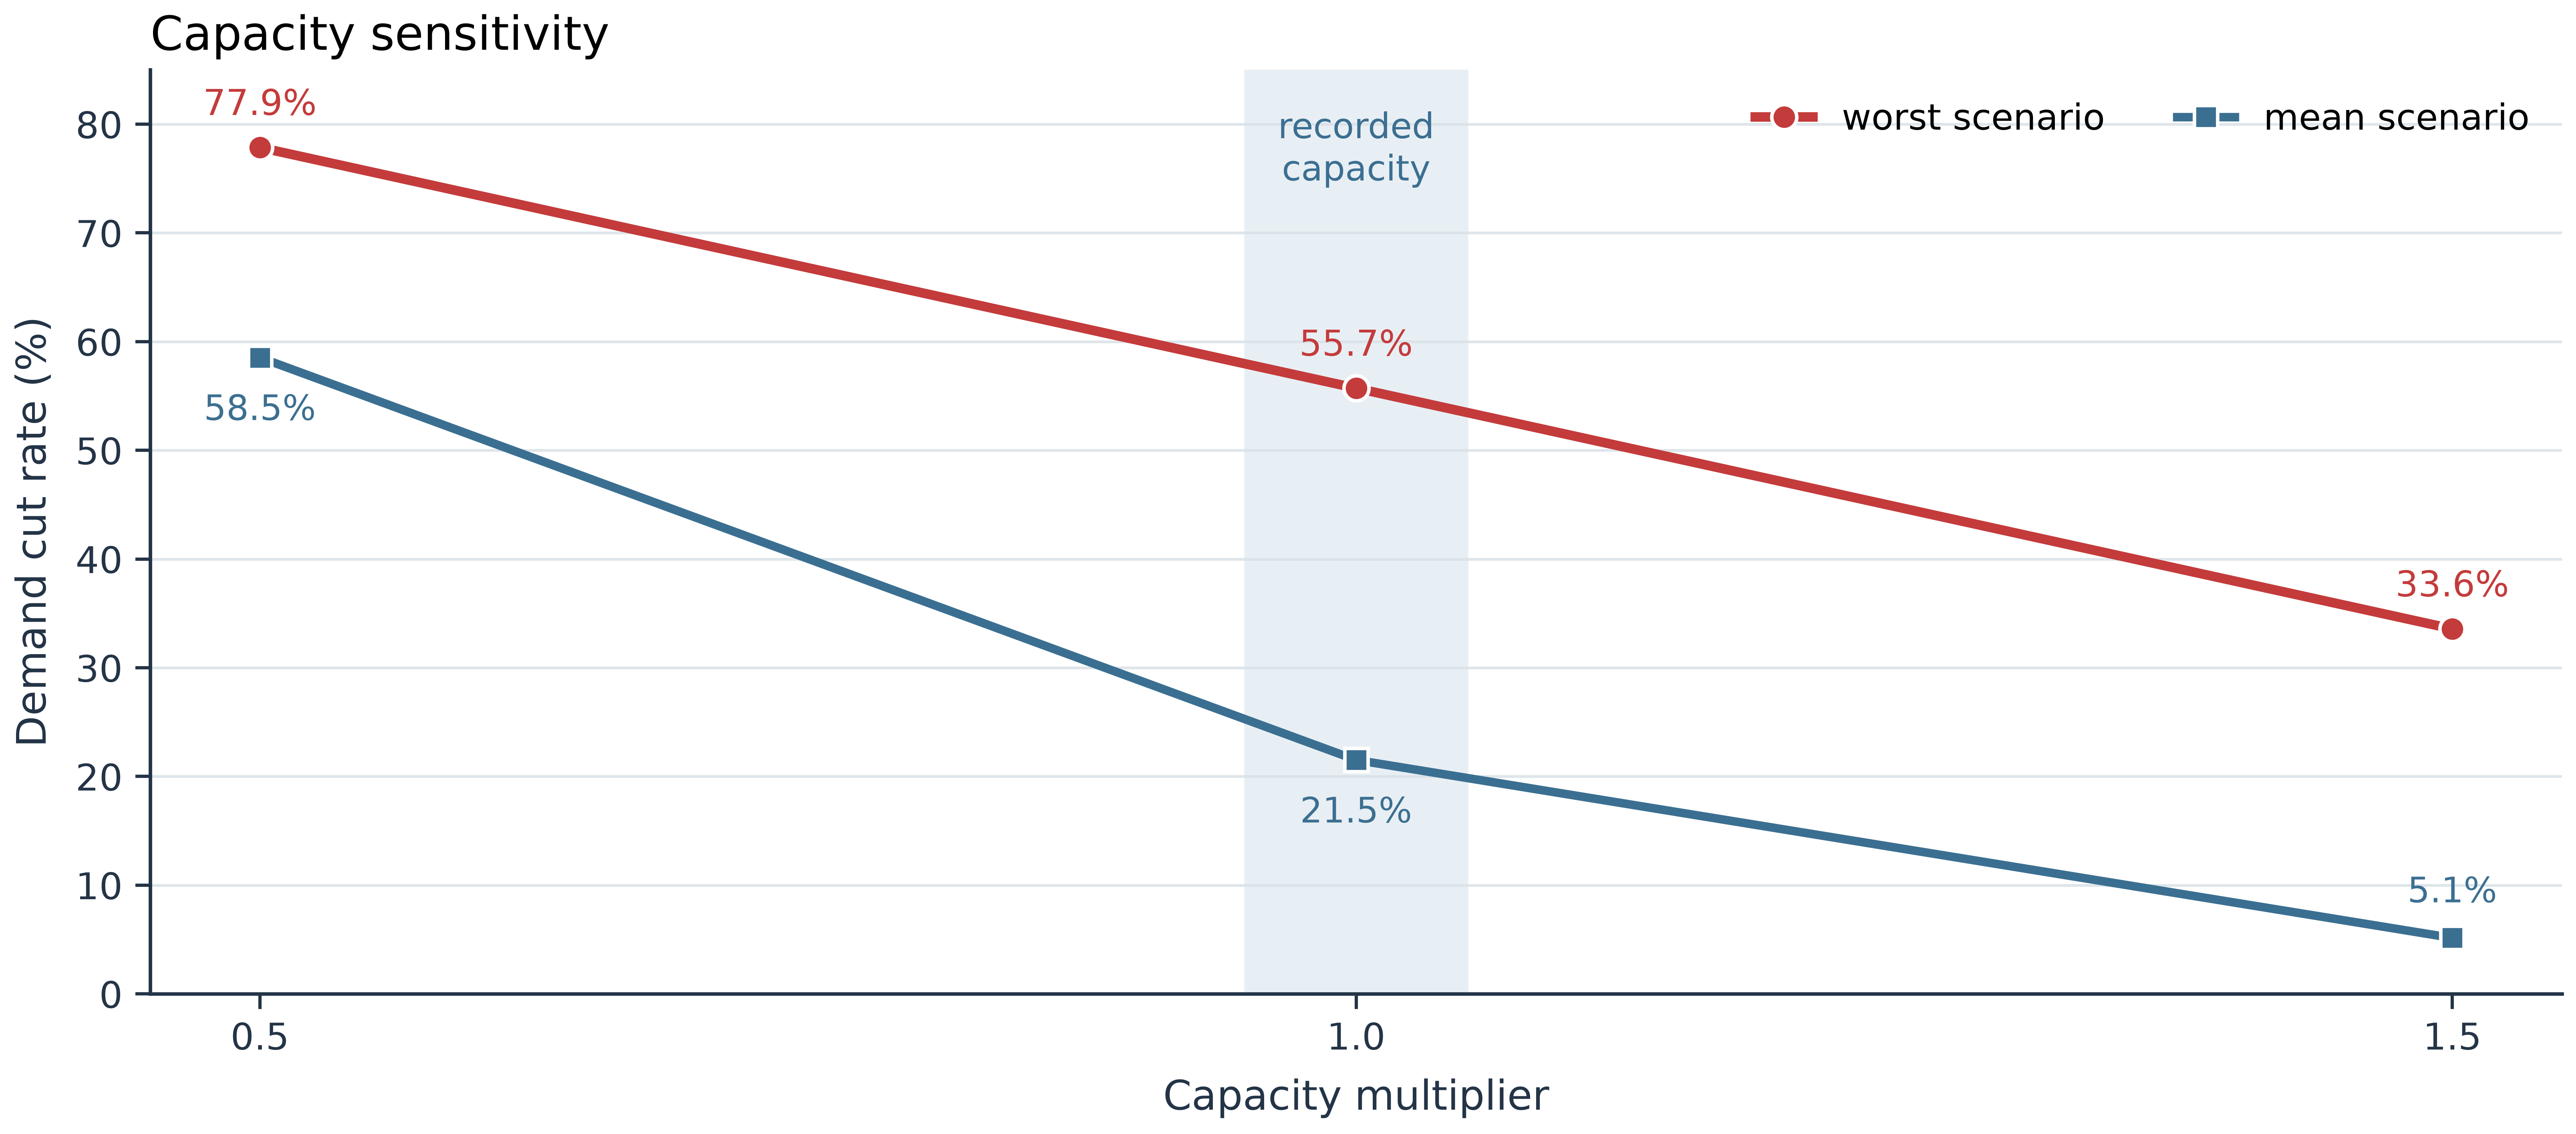
\includegraphics[width=0.98\textwidth]{figure6_capacity_sensitivity.png}
\caption{Demand curtailment under capacity scaling. The red series is the worst planning scenario and the blue series is the scenario mean. The shaded band marks the recorded capacity multiplier.}
\label{fig:capacity}
\end{figure*}

Figure~\ref{fig:external} compares the selected interface countries with the external TYNDP Hydrogen import targets. Panel (a) reports the top four country overlap and its predefined minimum. Panel (b) reports weighted target coverage. The overlap is two of the external top four in both 2030 and 2040, indicating partial alignment between the two constructs without implying replication.

\begin{figure*}[t]
\centering
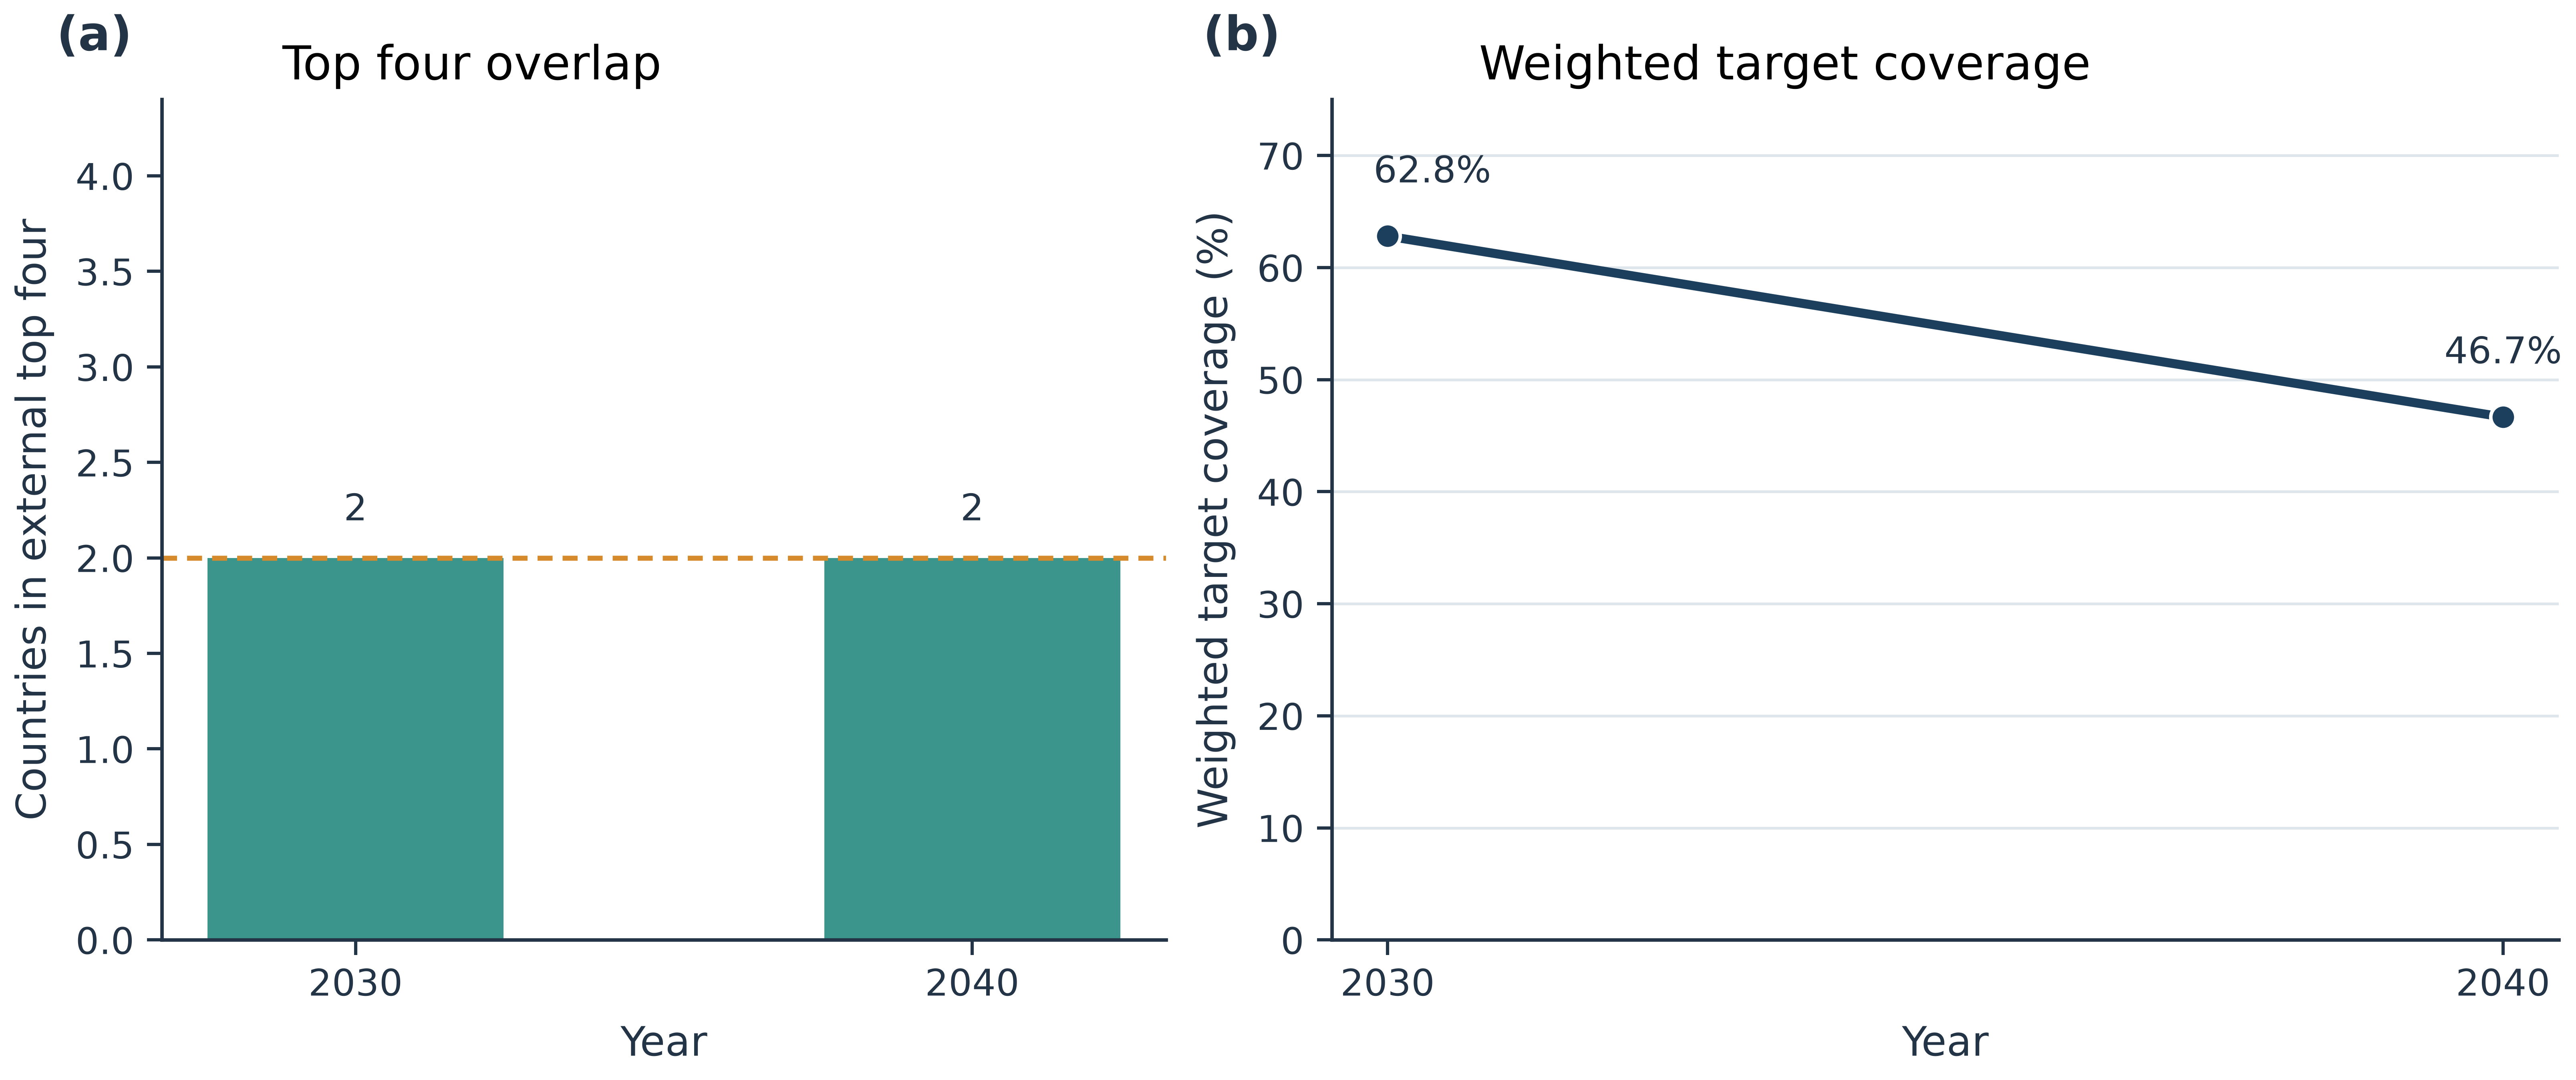
\includegraphics[width=0.98\textwidth]{figure7_external_face_validity.png}
\caption{External corridor face validity. (a) Overlap between the selected countries and the external top four targets, with the predefined minimum shown. (b) Weighted coverage of external targets in 2030 and 2040.}
\label{fig:external}
\end{figure*}

\section{Engineering Discussion}
\label{sec:discussion}

\subsection{Implications for practitioners}

The tool supports a fixed verification budget. A port or network planning team can use the ranked interface set to allocate the next limited round of endpoint, capacity, and compatibility checks, while retaining the scenario specific flow allocation as an engineering diagnostic. In the present product, explicit capacity evidence should be checked before carrier labels or the selected demand envelope because its removal increases N--1 failure stress by 22.11 percentage points.

The tool also supports scenario stress testing without changing the decision logic. Planners can rerun the same inventory for the 2030 and 2040 horizons, the PCI/PMI and Advanced infrastructure levels, and the low, medium, and high EHO demand envelopes. The result can therefore serve as a lightweight front end to a national or TYNDP planning study, followed by detailed route design, temporal network simulation, permitting review, and financial appraisal.

The interface budget is a verification budget. The main result uses four checks because it is the exact census budget. A supporting six interface run selects the same four core groups plus documented German and Polish candidates and retains the 55.72\% worst planning scenario rate. This sensitivity shows that the core priority set is not an artifact of the four interface reporting budget. The six interface result remains a verification resource allocation, while construction decisions require a separate investment study. The project graph also provides a transparent reason to avoid a country centroid shortcut: the star LP appears less constrained because it removes path and interface restrictions.

\subsection{Geographic concentration and scope}

The four interface result is concentrated in Belgium, Germany, northern France, and the Netherlands. The paper treats this as a property of the frozen candidate graph, shared pools, reachable facility accounting, and four interface budget, rather than as a geographic discovery. Italy and Poland are present in the source facility and project inventories, and Italy has an explicit candidate group; the selected set ranks candidates within the stated evidence and budget. The external corridor face check provides a second bounded perspective: two of the selected countries overlap the external top four in both 2030 and 2040. The practical contribution is the auditable selection and evidence gap ranking, which can be rerun when southern or eastern interface records gain endpoint and capacity evidence.

\subsection{Interpretation boundary}

The selected interfaces are verification priorities. Their modeled capacity ratios represent screening values, and the N--1/N--2 values are failure stress diagnostics for the declared scenarios. Operational throughput, queueing, storage, temporal balancing, local delivery routes, commercial return, and construction decisions require the evidence layers specified in the scope statement. The scenario based robust and deterministic selectors coincide in the main run; the scenario based robust formulation is consequently interpreted as a disciplined common scenario screening protocol, with its value demonstrated by exact portfolio discrimination, evidence gap detection, and transparent stress tests.

\subsection{Limitations and boundary conditions}

The most important limitation is data selection: public project lists may omit private or early stage assets. The exclusion ledger protects against unsupported imputation and can make the screen conservative. The second limitation is model specification: facility demand is allocated using published weights rather than a measured pipe level dispatch, and storage or temporal balancing require an additional model layer. The third limitation is construct mismatch: the external TYNDP Hydrogen import targets and the present interface priorities are different estimands. We report partial overlap and reserve replication claims for a construct aligned comparison.

\section{Reproducibility and Data Availability}
\label{sec:repro}

The accompanying package contains the frozen tabular data product, source manifest, exclusion records, the Natural Earth visualization asset used only as a light country backdrop, model code, figures, and fixed run outputs. The reported random portfolio diagnostic uses a fixed seed. Both the four interface main result and the six interface sensitivity result are included.

The MILP is solved with the open source \texttt{scipy.optimize.milp} implementation in the SciPy scientific computing stack \cite{Virtanen2020}.

The public raw source files remain available from their original repositories. The TYNDP 2024 data page and Hydrogen input archive are provided by ENTSOG; the larger PyPSA Eur TYNDP 2024 bundle is archived by Zenodo \cite{TYNDPZenodo}. EHB and JRC IDEES are cited as contextual and future extension sources. Restricted or oversized external source bundles remain at their original repositories.

\hyphenpenalty=10000
\exhyphenpenalty=10000
\emergencystretch=1em

\section{Conclusion}
\label{sec:conclusion}

This paper delivers a pre feasibility engineering screening tool with three practical outputs:
\begin{itemize}
\item \textbf{Verification priority list:} the exact equal budget census identifies four interfaces in Belgium, Germany, northern France, and the Netherlands. The worst planning scenario curtailment rate is 55.72\%, which is 22.18 percentage points below the equal budget median.
\item \textbf{Data collection priority:} withholding explicit capacity evidence raises N--1 failure stress by 22.11 percentage points. Capacity documentation is the first evidence collection priority in this product.
\item \textbf{Reusable planning screen:} the directed project graph, carrier compatible shared pools, lexicographic MILP, exact census, failure stress tests, and budget reruns form a repeatable what if protocol for port and hydrogen network planners.
\end{itemize}

The scope statement defines the interpretation of the selected interfaces. They are verification priorities, and operational throughput, temporal reliability, finance, and construction decisions require a subsequent evidence layer. Within this scope, all predefined diagnostic gates pass and the artifact provides a positive, auditable starting point for detailed engineering verification.

This paper contributes a reproducible, auditable screening protocol that translates public infrastructure records into a ranked verification set and an evidence gap diagnosis, enabling port and network planners to allocate verification resources before commissioning detailed engineering studies.


\hyphenpenalty=50
\exhyphenpenalty=50
\emergencystretch=0pt
\begin{thebibliography}{99}

\bibitem{EC_REPowerEU}
European Commission, "REPowerEU plan," COM(2022) 230 final, 2022. [Online]. Available: \url{https://eur-lex.europa.eu/legal-content/EN/TXT/?uri=COM:2022:230:FIN}

\bibitem{REDIII}
European Parliament and Council, "Directive (EU) 2023/2413," Official Journal of the European Union, 2023. [Online]. Available: \url{https://eur-lex.europa.eu/eli/dir/2023/2413/oj}

\bibitem{HydrogenRegulation}
European Parliament and Council, "Regulation (EU) 2024/1789 on the internal markets for renewable gas, natural gas, and hydrogen," Official Journal of the European Union, 2024. [Online]. Available: \url{https://eur-lex.europa.eu/eli/reg/2024/1789/oj}

\bibitem{HydrogenDirective}
European Parliament and Council, "Directive (EU) 2024/1788 on common rules for the internal markets for renewable gas, natural gas, and hydrogen," Official Journal of the European Union, 2024. [Online]. Available: \url{https://eur-lex.europa.eu/eli/dir/2024/1788/oj}

\bibitem{TENE}
European Parliament and Council, "Regulation (EU) 2022/869 on guidelines for trans-European energy infrastructure," Official Journal of the European Union, 2022. [Online]. Available: \url{https://eur-lex.europa.eu/eli/reg/2022/869/oj}

\bibitem{FuelEUMaritime}
European Parliament and Council, "Regulation (EU) 2023/1805 on the use of renewable and low-carbon fuels in maritime transport, and amending Directive 2009/16/EC," Official Journal of the European Union, 2023. [Online]. Available: \url{https://eur-lex.europa.eu/eli/reg/2023/1805/oj}

\bibitem{Raab2021}
M. Raab, S. Maier, and R.-U. Dietrich, "Comparative techno-economic assessment of a large-scale hydrogen transport via liquid transport media," \emph{Int. J. Hydrogen Energy}, vol. 46, pp. 11956--11968, 2021, doi: 10.1016/j.ijhydene.2020.12.213.

\bibitem{Johnston2022}
C. Johnston, M. H. A. Khan, R. Amal, R. Daiyan, and I. MacGill, "Shipping the sunshine: An open-source model for costing renewable hydrogen transport from Australia," \emph{Int. J. Hydrogen Energy}, vol. 47, pp. 20362--20377, 2022, doi: 10.1016/j.ijhydene.2022.04.156.

\bibitem{Lee2022}
J.-S. Lee \emph{et al.}, "Large-scale overseas transportation of hydrogen: Comparative techno-economic and environmental investigation," \emph{Renew. Sustain. Energy Rev.}, vol. 165, Art. no. 112556, 2022, doi: 10.1016/j.rser.2022.112556.

\bibitem{Sterner2024}
M. Sterner \emph{et al.}, "19 import options for green hydrogen and derivatives: An overview of efficiencies and technology readiness levels," \emph{Int. J. Hydrogen Energy}, vol. 90, pp. 1112--1127, 2024, doi: 10.1016/j.ijhydene.2024.10.045.

\bibitem{RestelliNH3}
F. Restelli \emph{et al.}, "Detailed techno-economic assessment of ammonia as green H2 carrier," \emph{Int. J. Hydrogen Energy}, vol. 52, pp. 532--547, 2024, doi: 10.1016/j.ijhydene.2023.06.206.

\bibitem{RestelliLH2}
F. Restelli \emph{et al.}, "Liquefied hydrogen value chain: A detailed techno-economic evaluation for its application in the industrial and mobility sectors," \emph{Int. J. Hydrogen Energy}, vol. 52, pp. 454--466, 2024, doi: 10.1016/j.ijhydene.2023.10.107.

\bibitem{Spatolisano2024}
E. Spatolisano \emph{et al.}, "Assessing opportunities and weaknesses of green hydrogen transport via LOHC through a detailed techno-economic analysis," \emph{Int. J. Hydrogen Energy}, vol. 52, pp. 703--717, 2024, doi: 10.1016/j.ijhydene.2023.08.040.

\bibitem{Peecock2024}
A. Peecock \emph{et al.}, "Techno-economic assessment of liquid carrier methods for intercontinental shipping of hydrogen: A case study," \emph{Int. J. Hydrogen Energy}, vol. 94, pp. 971--983, 2024, doi: 10.1016/j.ijhydene.2024.11.205.

\bibitem{Wolf2024}
N. Wolf, L. K\"uhn, and M. H\"ock, "International supply chains for a hydrogen ramp-up: Techno-economic assessment of hydrogen transport routes to Germany," \emph{Energy Conversion and Management: X}, vol. 23, Art. no. 100682, 2024, doi: 10.1016/j.ecmx.2024.100682.

\bibitem{Ganter2024}
A. Ganter, P. Gabrielli, and G. Sansavini, "Near-term infrastructure rollout and investment strategies for net-zero hydrogen supply chains," \emph{Renew. Sustain. Energy Rev.}, vol. 194, Art. no. 114314, 2024, doi: 10.1016/j.rser.2024.114314.

\bibitem{Kountouris2024}
I. Kountouris \emph{et al.}, "A unified European hydrogen infrastructure planning to support the rapid scale-up of hydrogen production," \emph{Nature Communications}, 2024, doi: 10.1038/s41467-024-49867-w.

\bibitem{Eissler2025}
T. Eissler \emph{et al.}, "Optimizing the supply chain for green hydrogen and derivatives: A case study from Australia to Germany including inland transport considerations," \emph{Int. J. Hydrogen Energy}, vol. 144, pp. 1200--1206, 2025, doi: 10.1016/j.ijhydene.2025.04.163.

\bibitem{Rey2025}
I. Rey, V. L. Barrio, and I. Agirre, "Environmental and economic assessment of large-scale hydrogen supply chains across Europe: LOHC versus other hydrogen technologies," \emph{Applied Energy}, vol. 401, Art. no. 126862, 2025, doi: 10.1016/j.apenergy.2025.126862.

\bibitem{GanterESNT2025}
A. Ganter, P. Gabrielli, H. Goericke, and G. Sansavini, "Minimum-regret hydrogen and carbon supply chains to decarbonize European industrial hydrogen demands," \emph{Environmental Science \& Technology}, 2025, doi: 10.1021/acs.est.4c13659.

\bibitem{He2021}
G. He, D. S. Mallapragada, A. Bose, C. F. Heuberger, and E. Gencer, "Hydrogen supply chain planning with flexible transmission and storage scheduling," \emph{IEEE Trans. Sustain. Energy}, vol. 12, no. 3, pp. 1730--1740, 2021, doi: 10.1109/TSTE.2021.3064015.

\bibitem{Jiang2022}
H. Jiang \emph{et al.}, "Modeling hydrogen supply chain in renewable electric energy system planning," \emph{IEEE Trans. Ind. Appl.}, vol. 58, no. 2, pp. 2780--2791, 2022, doi: 10.1109/TIA.2021.3117748.

\bibitem{Sadiq2021}
M. Sadiq \emph{et al.}, "Future greener seaports: A review of new infrastructure, challenges, and energy efficiency measures," \emph{IEEE Access}, vol. 9, pp. 75568--75587, 2021, doi: 10.1109/ACCESS.2021.3081430.

\bibitem{Paula2025}
K. F. Paula \emph{et al.}, "GIS-based Fuzzy-AHP framework for identifying suitable hubs for offshore wind and clean hydrogen production," \emph{IEEE Access}, vol. 13, pp. 65526--65539, 2025, doi: 10.1109/ACCESS.2025.3553704.

\bibitem{LuoHIES2023}
W. Luo, J. Wu, J. Cai, Y. Mao, and S. Chen, "Capacity allocation optimization framework for hydrogen integrated energy system considering hydrogen trading and long-term hydrogen storage," \emph{IEEE Access}, vol. 11, pp. 15772--15787, 2023, doi: 10.1109/ACCESS.2022.3228014.

\bibitem{BertsimasSim}
D. Bertsimas and M. Sim, "The price of robustness," \emph{Operations Research}, vol. 52, no. 1, pp. 35--53, 2004, doi: 10.1287/opre.1030.0065.

\bibitem{BenTalRobust}
A. Ben-Tal, L. El Ghaoui, and A. Nemirovski, \emph{Robust Optimization}. Princeton, NJ, USA: Princeton Univ. Press, 2009.

\bibitem{ENTSOGDownloads}
ENTSOG, "TYNDP 2024 downloads," 2024. [Online]. Available: \url{https://tyndp2024.entsog.eu/downloads/}

\bibitem{ENTSOGInfraLevels}
ENTSOG, "Hydrogen infrastructure levels," TYNDP 2024 H2 IGI report, 2024. [Online]. Available: \url{https://tyndp2024.entsog.eu/h2igi-report/hydrogen-infrastructure-levels/}

\bibitem{ENTSOGIGI}
ENTSOG, "Infrastructure gaps identification indicators," TYNDP 2024 H2 IGI report, 2024. [Online]. Available: \url{https://tyndp2024.entsog.eu/h2igi-report/infrastructure-gaps-identification-igi-indicators/}

\bibitem{ENTSOGAnnexA}
ENTSOG, "TYNDP 2024 Annex A: List of projects," 2024. [Online]. Available: \url{https://tyndp2024.entsog.eu/downloads/}

\bibitem{ENTSOGAnnexC2}
ENTSOG, "TYNDP 2024 Annex C2: Hydrogen infrastructure capacities," 2024. [Online]. Available: \url{https://tyndp2024.entsog.eu/downloads/}

\bibitem{ENTSOGHydrogenInputs}
ENTSOG, "Hydrogen import and generator properties workbook," TYNDP 2024 data archive, 2024. [Online]. Available: \url{https://2024-data.entsog-tyndp-scenarios.eu/files/scenarios-inputs/Hydrogen.zip}, accessed: Sep. 7, 2026.

\bibitem{EHOdemand}
European Hydrogen Observatory, "Hydrogen demand," 2025. [Online]. Available: \url{https://observatory.clean-hydrogen.europa.eu/hydrogen-landscape/end-use/hydrogen-demand}

\bibitem{EHOfuture}
European Hydrogen Observatory, "Scenarios for future hydrogen demand," 2023. [Online]. Available: \url{https://observatory.clean-hydrogen.europa.eu/tools-reports/scenarios-future-hydrogen-demand}

\bibitem{CHPPorts}
Clean Hydrogen Partnership, "Study on hydrogen ports and industrial coastal areas," 2023. [Online]. Available: \url{https://www.clean-hydrogen.europa.eu/media/publications/study-hydrogen-ports-and-industrial-coastal-areas-reports_en}

\bibitem{EHB}
European Hydrogen Backbone, "Implementation roadmap: Public support as catalyst for hydrogen infrastructure," 2024. [Online]. Available: \href{https://ehb.eu/files/downloads/1712733755_EHB-Implementation-Roadmap-Public-support-as-catalyst-for-hydrogen-infrastructure.pdf}{EHB implementation roadmap (PDF)}

\bibitem{JRCIDEES}
European Commission Joint Research Centre, "JRC IDEES 2021," European Commission data catalogue, 2024. [Online]. Available: \url{https://data.jrc.ec.europa.eu/dataset/1f0b480c-6d21-4d95-897d-20c7ca33df6f}

\bibitem{EurostatEnergy}
Eurostat, "Electricity prices for non-household consumers, nrg\_pc\_205," 2022. [Online]. Available: \url{https://ec.europa.eu/eurostat/api/dissemination/statistics/1.0/data/nrg_pc_205}

\bibitem{NaturalEarth}
Natural Earth, "1:110m cultural vectors: Admin 0 countries," public-domain cartographic data, accessed 2026. [Online]. Available: \url{https://github.com/nvkelso/natural-earth-vector/blob/master/geojson/ne_110m_admin_0_countries.geojson}

\bibitem{Virtanen2020}
P. Virtanen \emph{et al.}, "SciPy 1.0: Fundamental algorithms for scientific computing in Python," \emph{Nature Methods}, vol. 17, pp. 261--272, 2020, doi: 10.1038/s41592-019-0686-2.

\bibitem{TYNDPZenodo}
PyPSA-Eur contributors, "TYNDP 2024 data bundle," Zenodo, 2024. [Online]. Available: \url{https://zenodo.org/records/14230568}

\end{thebibliography}
\section*{Declaration of Generative AI and AI-assisted Technologies}
OpenAI Codex was used for Python code debugging and English-language editing during manuscript preparation. No AI-generated tables, figures, statistical results, or substantive claims are included in this manuscript. The authors reviewed and verified all source records, transformations, code outputs, and interpretations and take full responsibility for the final manuscript.

\begin{IEEEbiographynophoto}{Ruojun Duan}
is affiliated with the School of Political Science and International Relations, Tongji University, Shanghai 200092, China. His research interests include public-data infrastructure screening, energy transition governance, and transparent decision-support systems.
\end{IEEEbiographynophoto}

\begin{IEEEbiographynophoto}{Junjie Zhang}
is a Ph.D. candidate with Shanghai International Studies University, Shanghai 201620, China. His research interests include hydrogen import infrastructure, public-data capacity screening, and energy-system planning.
\end{IEEEbiographynophoto}

\EOD
\end{document}
